\documentclass[UTF8,11pt]{ctexart}
\usepackage[a4paper,margin=19mm]{geometry}
\usepackage{amsmath,amssymb,tikz,graphicx,hyperref}
\usetikzlibrary{arrows.meta,decorations.pathmorphing}
\setlength{\parindent}{0pt}\setlength{\parskip}{6pt}
\sloppy\emergencystretch=3em

% Site layout only: preserve text, mathematics and native chemical diagrams.
\setlength{\parskip}{2pt}
\raggedbottom
\let\originalenumerate\enumerate
\renewcommand{\enumerate}{\originalenumerate
 \setlength{\itemsep}{2pt}\setlength{\parsep}{0pt}\setlength{\topsep}{3pt}}
\makeatletter
\renewcommand\subsection{\@startsection{subsection}{2}{\z@}
 {-1.1ex\@plus -.3ex\@minus -.2ex}{.5ex\@plus .2ex}
 {\normalfont\normalsize\bfseries}}
\makeatother

\begin{document}\newsavebox{\mockquestionbox}
\begin{center}{\LARGE 南京工业大学637有机化学}\par\medskip{\Large D19 近期型模拟卷 详细解析}\par\medskip 满分150分\quad 考试时间180分钟\end{center}本解析供交卷后核对。采分点为训练建议，不是学校官方评分。等效、化学成立且满足题限的解法应酌情给分。\par\section*{一、填空、命名与完成反应（15题，共30分）}\subsection*{1．（2分）}请写出下列化合物的中、英文系统名称。\[\mathrm{CH_3CH_2CH_2CH(CH_2CH_3)C(CH_3)_2CH_2CH_2CH_2CH_3}\]\subsection*{答案与结构}中文：5,5-二甲基-4-乙基壬烷；英文：4-ethyl-5,5-dimethylnonane。\subsection*{从概念到解法}\begin{enumerate}\item 系统命名先确定连续最长碳链。图中从左端经支化点、季碳到右端共有9个碳，故母体是壬烷，不能只因支链多便选短链。\item 从左编号得到支链位次4,5,5；反向得到5,5,6，第一差异处4小于5，所以采用前者。\item 4位为乙基，5位有两个甲基。中文按本教材习惯列甲基、乙基；英文按ethyl、methyl字母顺序排列，di不参与字母排序。\end{enumerate}\subsection*{验算与易错}碳数9+2+2=13，重写名称能还原原连接。；编号方向比较的是排序后的位次序列，不是位次总和。\subsection*{参考采分（非官方）}中文1分；英文1分。\par 来源：S01，2-7(i)，印刷页10，PDF页16。\par\medskip\clearpage\subsection*{2．（2分）}计算下面分子的旋光异构体的数目。有几对对映体？每一个化合物有几个非对映体？\begin{center}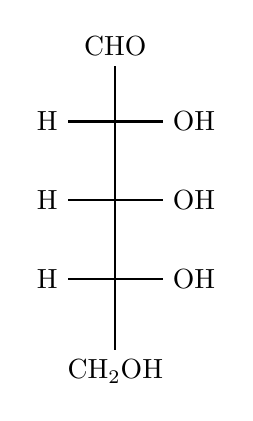
\begin{tikzpicture}[line width=.85pt,>=Stealth]\draw(0,1)--(0,-2.6);\node[above]at(0,1){$\mathrm{CHO}$};\node[below]at(0,-2.6){$\mathrm{CH_2OH}$};\draw(-.6,0.3)--(.6,0.3);\node[left]at(-.6,0.3){$\mathrm{H}$};\node[right]at(.6,0.3){$\mathrm{OH}$};\draw(-.6,-0.7)--(.6,-0.7);\node[left]at(-.6,-0.7){$\mathrm{H}$};\node[right]at(.6,-0.7){$\mathrm{OH}$};\draw(-.6,-1.7)--(.6,-1.7);\node[left]at(-.6,-1.7){$\mathrm{H}$};\node[right]at(.6,-1.7){$\mathrm{OH}$};\end{tikzpicture}\end{center}\subsection*{答案与结构}共有8个构型异构体，构成4对对映体；每个构型异构体各有6个非对映体。\subsection*{从概念到解法}\begin{enumerate}\item 手性碳连四个不同基团。开链醛糖的三个交叉点均满足该条件，故有3个独立立体中心。\item 先列2的3次方=8种R/S组合。上端CHO与下端CH2OH不同，整条链没有使端基互换后仍相同的内部对称性，不能再扣去内消旋体。\item 一个构型的三个中心全部反转得其唯一镜像。8个分子两两配对，共4对。\item 固定一个异构体，排除它自己和其对映体，余8-2=6个均为非对映体。Fischer横键向前、竖键向后；整图转90度不能当作同一构型。\end{enumerate}\subsection*{验算与易错}三个中心都反转才是镜像；部分反转是非对映关系。；链两端不同，无meso造成的计数合并。\subsection*{参考采分（非官方）}8个0.75分；4对0.5分；每个6个0.75分。\par 来源：S01，3-16，印刷页32，PDF页38。\par\medskip\clearpage\subsection*{3．（2分）}1-己炔在$3305\,\mathrm{cm^{-1}}$、$2110\,\mathrm{cm^{-1}}$、$620\,\mathrm{cm^{-1}}$处有吸收峰。指出这三个吸收峰的归属。\subsection*{答案与结构}$3305\,\mathrm{cm^{-1}}$：末端$\mathrm{\equiv C-H}$伸缩；$2110\,\mathrm{cm^{-1}}$：$\mathrm{C\equiv C}$伸缩；$620\,\mathrm{cm^{-1}}$：末端$\mathrm{\equiv C-H}$弯曲振动。\subsection*{从概念到解法}\begin{enumerate}\item 红外吸收对应引起偶极矩变化的分子振动。较强、较短的键，其伸缩振动通常位于较高波数。\item 1-己炔是末端炔，兼有sp碳上的C-H和碳碳三键。高波数3305归给sp C-H伸缩；2110处于三键伸缩区。\item 620是较低频弯曲，不能再写为C-H伸缩。题目已给出化合物身份，只需归属，不应把它改成未知结构推断。\end{enumerate}\subsection*{验算与易错}峰位是本题给定数据，不宣称所有端炔都恰为这三个数值。；伸缩与弯曲区分完整，未把三键写为烯键。\subsection*{参考采分（非官方）}两处伸缩各0.75分；弯曲0.5分。\par 来源：S01，5-25，印刷页60，PDF页66。\par\medskip\clearpage\subsection*{4．（2分）}写出下列离子发生分子内$\mathrm{S_N2}$反应的反应产物。\begin{center}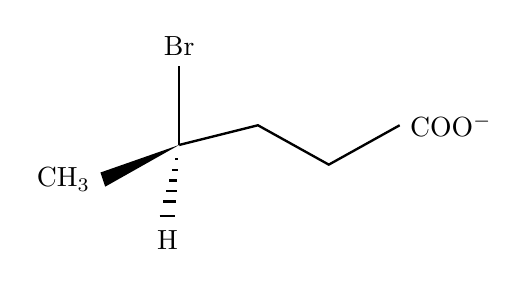
\begin{tikzpicture}[line width=.85pt,>=Stealth]\coordinate(c)at(0,0);\draw(c)--(0,1)node[above]{$\mathrm{Br}$};\draw(c)--(1,.25)--(1.9,-.25)--(2.8,.25);\node[right]at(2.8,.25){$\mathrm{COO^-}$};\fill(c)--(-1,-.35)--(-.94,-.53)--cycle;\node[left]at(-1,-.44){$\mathrm{CH_3}$};\foreach\t in{.2,.35,.5,.65,.8,1}{\draw(-.15*\t-.1*\t,-.9*\t)--(-.15*\t+.1*\t,-.9*\t);}\node[below]at(-.15,-.95){$\mathrm{H}$};\end{tikzpicture}\end{center}\subsection*{答案与结构}生成$(5S)$-5-甲基氧杂环戊烷-2-酮（该图所示单一构型），另有$\mathrm{Br^-}$离去。\begin{center}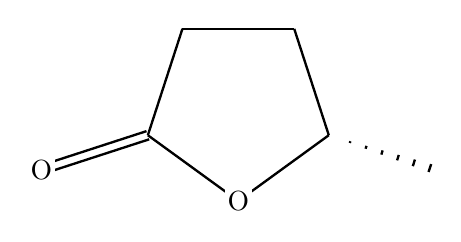
\begin{tikzpicture}[line width=.85pt,>=Stealth]\draw (1.416,-0.356)--(1.423,-0.335);
\draw (1.616,-0.430)--(1.628,-0.393);
\draw (1.816,-0.504)--(1.833,-0.451);
\draw (2.016,-0.577)--(2.038,-0.509);
\draw (2.216,-0.651)--(2.243,-0.567);
\draw (2.416,-0.725)--(2.449,-0.625);
\draw (1.149,-0.258)--(0.710,1.093);
\draw (0.710,1.093)--(-0.710,1.093);
\draw (-0.710,1.093)--(-1.149,-0.258);
\draw (-1.166,-0.206)--(-2.517,-0.645);
\draw (-1.132,-0.310)--(-2.483,-0.749);
\draw (-1.149,-0.258)--(-0.000,-1.093);
\draw (-0.000,-1.093)--(1.149,-0.258);
\node[fill=white,inner sep=1.1pt]at(-2.500,-0.697){$\mathrm{O}$};
\node[fill=white,inner sep=1.1pt]at(-0.000,-1.093){$\mathrm{O}$};\end{tikzpicture}\end{center}\subsection*{从概念到解法}\begin{enumerate}\item 羧酸根O带孤对与负电，是分子内亲核位点；连Br的碳是亲电中心。沿O、反应中心、两个CH2、羰基碳数环，闭合为五元内酯。\item 羧酸根O从C-Br键背面进攻，成C-O与断C-Br协同进行，不画自由碳正离子。\item 原图Br优先于羧酸端碳链，碳链优先于Me，H为最低优先级；H向后，原中心为R。产物O、环碳链、Me、H次序下为S，体现背面进攻的几何翻转。\item 只有一个指定立体底物，不能无理由写成外消旋；也不能把原有Me键不变地抄到随意旋转后的平面环而丢失构型。\end{enumerate}\subsection*{验算与易错}反应中心前后总碳数均5。；产物C5H8O2加Br负离子与原离子的原子、电荷匹配。；RDKit只辅助检查S标签和价态，SN2背面进攻由人工化学推导。\subsection*{参考采分（非官方）}五元内酯连接1分；正确翻转构型1分。\par 来源：S01，6-16(ii)，印刷页85，PDF页91。\par\medskip\clearpage\subsection*{5．（2分）}完成下列反应，写出产物。\begin{center}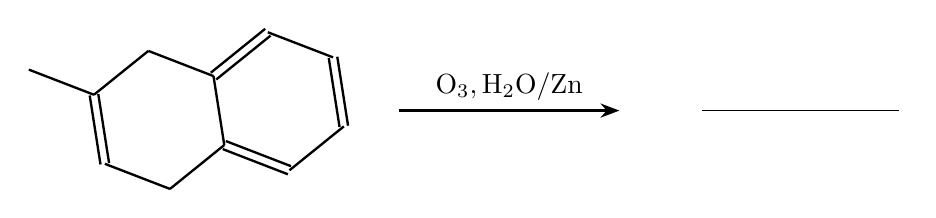
\begin{tikzpicture}[line width=.85pt,>=Stealth]\draw (-2.000,0.520)--(-1.173,0.201);
\draw (-1.227,0.192)--(-1.090,-0.684);
\draw (-1.118,0.209)--(-0.981,-0.667);
\draw (-1.035,-0.676)--(-0.208,-0.995);
\draw (-0.208,-0.995)--(0.482,-0.438);
\draw (0.462,-0.489)--(1.290,-0.809);
\draw (0.502,-0.387)--(1.329,-0.706);
\draw (1.310,-0.758)--(2.000,-0.201);
\draw (2.054,-0.192)--(1.917,0.684);
\draw (1.946,-0.209)--(1.809,0.667);
\draw (1.863,0.676)--(1.035,0.995);
\draw (1.001,1.038)--(0.311,0.481);
\draw (1.070,0.952)--(0.380,0.395);
\draw (0.345,0.438)--(-0.482,0.758);
\draw (-0.482,0.758)--(-1.173,0.201);
\draw (0.345,0.438)--(0.482,-0.438);\draw[->](2.7,0)--(5.5,0)node[midway,above,align=center]{$\mathrm{O_3,H_2O/Zn}$};\node at(7.8,0){\rule{2.5cm}{.3pt}};\end{tikzpicture}\end{center}\subsection*{答案与结构}非芳烯键还原臭氧裂解后为邻位分别带CH2CHO及CH2COCH3的苯：2-(2-氧代丙基)苯乙醛。\begin{center}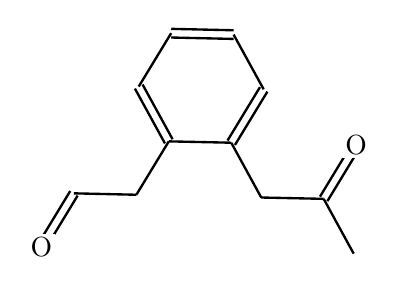
\begin{tikzpicture}[line width=.85pt,>=Stealth]\draw (1.967,-1.400)--(1.586,-0.704);
\draw (1.633,-0.733)--(2.045,-0.055);
\draw (1.539,-0.676)--(1.951,0.002);
\draw (1.586,-0.704)--(0.793,-0.687);
\draw (0.793,-0.687)--(0.412,0.009);
\draw (0.459,-0.020)--(0.871,0.658);
\draw (0.365,0.037)--(0.777,0.715);
\draw (0.824,0.687)--(0.442,1.382);
\draw (0.443,1.437)--(-0.350,1.455);
\draw (0.441,1.327)--(-0.352,1.345);
\draw (-0.351,1.400)--(-0.763,0.722);
\draw (-0.811,0.696)--(-0.430,-0.000);
\draw (-0.714,0.748)--(-0.333,0.053);
\draw (-0.381,0.026)--(-0.793,-0.652);
\draw (-0.793,-0.652)--(-1.586,-0.634);
\draw (-1.633,-0.605)--(-2.045,-1.283);
\draw (-1.539,-0.663)--(-1.951,-1.341);
\draw (-0.381,0.026)--(0.412,0.009);
\node[fill=white,inner sep=1.1pt]at(1.998,-0.026){$\mathrm{O}$};
\node[fill=white,inner sep=1.1pt]at(-1.998,-1.312){$\mathrm{O}$};\end{tikzpicture}\end{center}\subsection*{从概念到解法}\begin{enumerate}\item 臭氧作用于图示非芳碳碳双键，Zn/H2O为还原处理；先在两个烯碳处断双键，每个烯碳各补一个O为羰基。\item 原带Me的烯碳无H，裂后为甲基酮端；另一个烯碳带H，裂后为醛端。\item 裂的是非芳六元环中的双键，芳苯环保留，两个侧链仍通过苯环连接。不能把整分子切成两个独立小分子，或在还原处理下自动把醛氧化为酸。\end{enumerate}\subsection*{验算与易错}C11H12到C11H12O2，增加2O而保留全部11C。；芳环保持六\(\pi\)体系；一醛一酮对应原双键一端有H一端无H。\subsection*{参考采分（非官方）}开环连接1分；醛酮端点正确1分。\par 来源：S02，模拟试题2·二·3，印刷页122，PDF页131。\par\medskip\clearpage\subsection*{6．（2分）}完成下列反应式，写出主要产物，并命名各步产物。\[\mathrm{CH_3CH_2CH_2CHO+NaHSO_3}\,(\text{饱和})\longrightarrow\boxed{\phantom{AAAA}}\xrightarrow{\mathrm{Na_2CO_3}}\boxed{\phantom{AAAA}}\]\subsection*{答案与结构}第一步为丁醛亚硫酸氢钠加合物$\mathrm{CH_3CH_2CH_2CH(OH)SO_3Na}$（1-羟基丁烷-1-磺酸钠）；第二步恢复丁醛$\mathrm{CH_3CH_2CH_2CHO}$。\begin{center}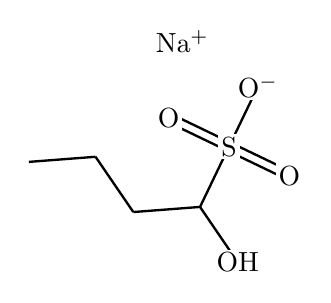
\begin{tikzpicture}[line width=.85pt,>=Stealth]\draw (-1.654,-0.126)--(-0.807,-0.061);
\draw (-0.807,-0.061)--(-0.327,-0.763);
\draw (-0.327,-0.763)--(0.520,-0.698);
\draw (0.520,-0.698)--(0.999,-1.400);
\draw (0.520,-0.698)--(0.888,0.068);
\draw (0.864,0.018)--(1.630,-0.350);
\draw (0.912,0.117)--(1.678,-0.251);
\draw (0.912,0.117)--(0.146,0.485);
\draw (0.864,0.018)--(0.098,0.386);
\draw (0.888,0.068)--(1.256,0.834);
\node[fill=white,inner sep=1.1pt]at(0.999,-1.400){$\mathrm{OH}$};
\node[fill=white,inner sep=1.1pt]at(0.888,0.068){$\mathrm{S}$};
\node[fill=white,inner sep=1.1pt]at(1.654,-0.300){$\mathrm{O}$};
\node[fill=white,inner sep=1.1pt]at(0.122,0.435){$\mathrm{O}$};
\node[fill=white,inner sep=1.1pt]at(1.256,0.834){$\mathrm{O^{-}}$};
\node[fill=white,inner sep=1.1pt]at(0.295,1.400){$\mathrm{Na^{+}}$};\end{tikzpicture}\end{center}\begin{center}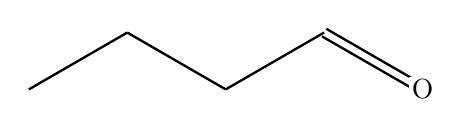
\begin{tikzpicture}[line width=.85pt,>=Stealth]\draw (-2.500,-0.361)--(-1.250,0.361);
\draw (-1.250,0.361)--(0.000,-0.361);
\draw (0.000,-0.361)--(1.250,0.361);
\draw (1.222,0.313)--(2.473,-0.408);
\draw (1.278,0.408)--(2.527,-0.313);
\node[fill=white,inner sep=1.1pt]at(2.500,-0.361){$\mathrm{O}$};\end{tikzpicture}\end{center}\subsection*{从概念到解法}\begin{enumerate}\item 羰基碳因C=O极化而缺电子，亚硫酸氢根在醛基碳形成C-S键，羰基O经质子转移成为OH；不能把它写成亚硫酸酯C-O-S连接。\item 加成反应可逆，碳酸钠使加合物分解释放原醛；没有把醛还原成醇，也没有增加底物碳数。\item 加合物新形成的碳连OH、磺酸盐、H、丙基，可能形成一对对映体；原题未指定绝对构型，不写成唯一R或S。\end{enumerate}\subsection*{验算与易错}第一步C4骨架保留，C-S非C-O-S。；碳酸钠不提供额外碳骨架，也不是本题还原剂。\subsection*{参考采分（非官方）}每步正确结构0.5分、正确名称0.5分。\par 来源：S01，10-15(i)，印刷页188，PDF页194。\par\medskip\clearpage\subsection*{7．（2分）}完成以下反应式：\begin{center}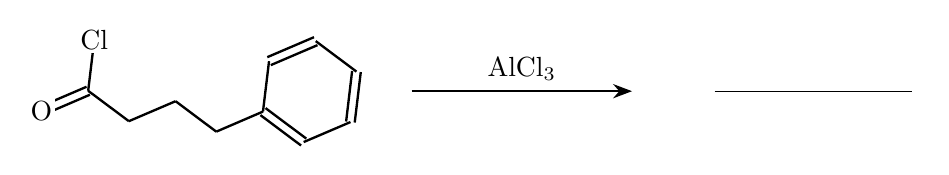
\begin{tikzpicture}[line width=.85pt,>=Stealth]\draw (-1.978,-0.300)--(-1.385,-0.045);
\draw (-2.022,-0.199)--(-1.428,0.056);
\draw (-1.407,0.005)--(-1.330,0.646);
\draw (-1.407,0.005)--(-0.890,-0.381);
\draw (-0.890,-0.381)--(-0.297,-0.127);
\draw (-0.297,-0.127)--(0.220,-0.514);
\draw (0.220,-0.514)--(0.813,-0.259);
\draw (0.781,-0.304)--(1.297,-0.690);
\draw (0.846,-0.215)--(1.363,-0.602);
\draw (1.330,-0.646)--(1.924,-0.392);
\draw (1.978,-0.398)--(2.055,0.243);
\draw (1.869,-0.385)--(1.945,0.256);
\draw (2.000,0.249)--(1.483,0.636);
\draw (1.461,0.686)--(0.868,0.432);
\draw (1.505,0.585)--(0.912,0.331);
\draw (0.890,0.381)--(0.813,-0.259);
\node[fill=white,inner sep=1.1pt]at(-2.000,-0.249){$\mathrm{O}$};
\node[fill=white,inner sep=1.1pt]at(-1.330,0.646){$\mathrm{Cl}$};\draw[->](2.7,0)--(5.5,0)node[midway,above,align=center]{$\mathrm{AlCl_3}$};\node at(7.8,0){\rule{2.5cm}{.3pt}};\end{tikzpicture}\end{center}\subsection*{答案与结构}产物为1-四氢萘酮（1-tetralone，结构如下）。\begin{center}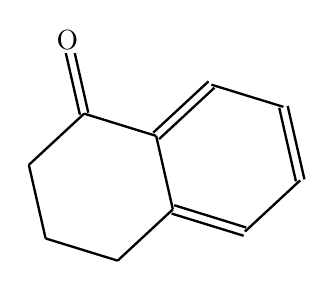
\begin{tikzpicture}[line width=.85pt,>=Stealth]\draw (-1.288,1.388)--(-1.075,0.454);
\draw (-1.180,1.412)--(-0.968,0.479);
\draw (-1.021,0.467)--(-1.723,-0.184);
\draw (-1.723,-0.184)--(-1.510,-1.118);
\draw (-1.510,-1.118)--(-0.595,-1.400);
\draw (-0.595,-1.400)--(0.106,-0.749);
\draw (0.090,-0.802)--(1.005,-1.084);
\draw (0.123,-0.696)--(1.037,-0.979);
\draw (1.021,-1.031)--(1.723,-0.380);
\draw (1.777,-0.368)--(1.564,0.565);
\draw (1.669,-0.393)--(1.457,0.541);
\draw (1.510,0.553)--(0.595,0.835);
\draw (0.558,0.876)--(-0.144,0.225);
\draw (0.633,0.795)--(-0.069,0.144);
\draw (-0.106,0.184)--(-1.021,0.467);
\draw (-0.106,0.184)--(0.106,-0.749);
\node[fill=white,inner sep=1.1pt]at(-1.234,1.400){$\mathrm{O}$};\end{tikzpicture}\end{center}\subsection*{从概念到解法}\begin{enumerate}\item AlCl3作为Lewis酸活化酰氯，使羰基碳成为强亲电位点。连到苯环的三个CH2与酰基碳形成可闭合的侧链。\item 邻位芳碳进攻酰基碳形成新C-C键；计数苯环邻位碳、连侧链芳碳、三个CH2、羰基碳，恰好六元环。\item 芳香亲电取代的\(\sigma\)络合物失去质子恢复苯环芳香性。酮O与AlCl3配位，通常经后处理释放酮；原题只印AlCl3，正式题干照录，不能把未印的水解试剂冒称原条件。\end{enumerate}\subsection*{验算与易错}起始C10到产物C10，净去HCl。；两个邻位因未取代苯环对称而等价，不产生两种位置异构体。；酰基无烷基正离子型骨架重排。\subsection*{参考采分（非官方）}六元稠环1分；羰基位置与苯环双键1分。\par 来源：S01，16-20(i)，印刷页326，PDF页332。\par\medskip\clearpage\subsection*{8．（2分）}S02-M02-一-Q01\quad 印刷121页 / PDF130页。\par\bigskip
用Fischer投影式表示$(R)$-3-羟基丁醛。
\par\medskip\textbf{答案：}图示Fischer投影。
\begin{center}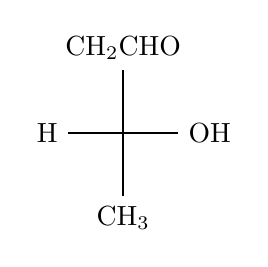
\begin{tikzpicture}[line width=.8pt]\draw(0,-.8)--(0,.8);\draw(-.7,0)--(.7,0);\node[above]at(0,.8){$\mathrm{CH_2CHO}$};\node[below]at(0,-.8){$\mathrm{CH_3}$};\node[left]at(-.7,0){$\mathrm H$};\node[right]at(.7,0){$\mathrm{OH}$};\end{tikzpicture}\end{center}
\textbf{推导与理由：}\begin{enumerate}\item 先按醛基最高优先级官能团从CHO端编号：CHO为C1，OH在C3。C3所连基团优先序为OH＞CH2CHO＞CH3＞H。
\item Fischer竖线指向纸后，横线指向读者。把CH2CHO放上、CH3放下，OH在右、H在左；图上1$\rightarrow$2$\rightarrow$3为逆时针，但最低H向前，需反向，得到R。\end{enumerate}
\textbf{反向验算与边界：}\begin{itemize}\item 四碳守恒；羟基未误移到C2；不是乳酸；横向H朝前已作反转。\end{itemize}
 原书答案对照：印刷125页。\par\medskip\clearpage\subsection*{9．（2分）}S02-M02-一-Q06\quad 印刷121页 / PDF130页。\par\bigskip
写出下列化合物的俗名。
\begin{center}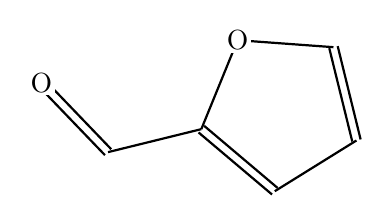
\begin{tikzpicture}[line width=.8pt]\draw (-2.040,0.379)--(-1.194,-0.501);
\draw (-1.960,0.455)--(-1.115,-0.425);
\draw (-1.155,-0.463)--(0.030,-0.171);
\draw (-0.005,-0.213)--(0.928,-1.001);
\draw (0.066,-0.129)--(0.998,-0.917);
\draw (0.963,-0.959)--(2.000,-0.315);
\draw (2.053,-0.302)--(1.762,0.883);
\draw (1.947,-0.328)--(1.655,0.857);
\draw (1.708,0.870)--(0.491,0.959);
\draw (0.491,0.959)--(0.030,-0.171);
\node[fill=white,inner sep=1.1pt]at(-2.000,0.417){$\mathrm{O}$};
\node[fill=white,inner sep=1.1pt]at(0.491,0.959){$\mathrm{O}$};\end{tikzpicture}\end{center}
\par\medskip\textbf{答案：}糠醛（呋喃-2-甲醛）。
\textbf{推导与理由：}\begin{enumerate}\item 识别五元含氧芳杂环为呋喃；醛基位于紧邻氧的2位。原题要求俗名，故答案应写糠醛，系统名只作辅助核对。\end{enumerate}
\textbf{反向验算与边界：}\begin{itemize}\item 醛基不是直接接在氧上；不是3-呋喃甲醛；保留CHO而不是COOH。\end{itemize}
 原书答案对照：印刷125页。\par\medskip\clearpage\subsection*{10．（2分）}S02-M03-一-Q04\quad 印刷129页 / PDF138页。\par\bigskip
完成下列反应，填入适当试剂。
\begin{center}\begin{tabular}{ccc}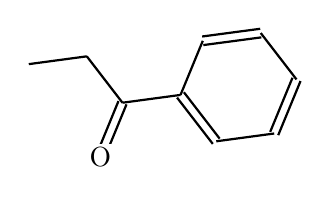
\begin{tikzpicture}[line width=.8pt]\draw (-1.700,0.391)--(-0.963,0.490);
\draw (-0.963,0.490)--(-0.510,-0.099);
\draw (-0.561,-0.078)--(-0.843,-0.765);
\draw (-0.459,-0.120)--(-0.742,-0.807);
\draw (-0.510,-0.099)--(0.227,-0.000);
\draw (0.183,-0.034)--(0.637,-0.622);
\draw (0.270,0.034)--(0.724,-0.555);
\draw (0.681,-0.589)--(1.417,-0.490);
\draw (1.468,-0.511)--(1.751,0.176);
\draw (1.366,-0.469)--(1.649,0.218);
\draw (1.700,0.197)--(1.246,0.786);
\draw (1.239,0.840)--(0.502,0.742);
\draw (1.254,0.731)--(0.517,0.633);
\draw (0.510,0.687)--(0.227,-0.000);
\node[fill=white,inner sep=1.1pt]at(-0.792,-0.786){$\mathrm{O}$};\end{tikzpicture}&$\xrightarrow{\text{（填试剂）}}$&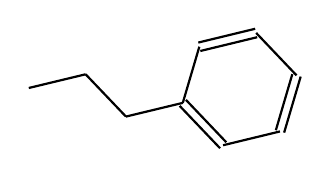
\begin{tikzpicture}[line width=.8pt]\draw (-1.700,0.014)--(-0.978,0.188);
\draw (-0.978,0.188)--(-0.466,-0.349);
\draw (-0.466,-0.349)--(0.256,-0.175);
\draw (0.216,-0.213)--(0.729,-0.751);
\draw (0.296,-0.137)--(0.808,-0.675);
\draw (0.768,-0.713)--(1.490,-0.538);
\draw (1.543,-0.553)--(1.753,0.159);
\draw (1.438,-0.522)--(1.647,0.190);
\draw (1.700,0.175)--(1.188,0.713);
\draw (1.175,0.766)--(0.453,0.591);
\draw (1.201,0.659)--(0.479,0.484);
\draw (0.466,0.538)--(0.256,-0.175);\end{tikzpicture}\end{tabular}\end{center}
\par\medskip\textbf{答案：}$\mathrm{Zn(Hg)/HCl}$；也可答$\mathrm{NH_2NH_2/KOH}$、加热。
\textbf{推导与理由：}\begin{enumerate}\item 比较起止结构：苯环和三碳侧链不变，只有C=O变为CH2，是羰基去氧还原。
\item 酸性Clemmensen还原可用锌汞齐/盐酸；本底物无明显酸敏感基团。碱性Wolff–Kishner条件也能实现相同净转化，不因原书只列一种而否认合理答案。\end{enumerate}
\textbf{反向验算与边界：}\begin{itemize}\item NaBH4或LiAlH4单独通常得醇，不直接给烃；不能用加氢把芳环一起还原；三碳侧链未缩短。\end{itemize}
 原书答案对照：印刷131页。\par\medskip\clearpage\subsection*{11．（2分）}原书：华东理工大学模拟试题（一） 一、回答问题 第25题；PDF[107]，印刷页[102]。\par\smallskip 完成反应，填写全部原空\par\smallskip \par\smallskip 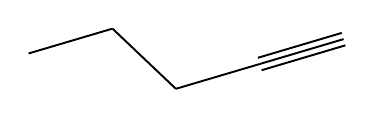
\begin{tikzpicture}[line width=.7pt]\draw (-2.000,0.067)--(-0.935,0.382);
\draw (-0.935,0.382)--(-0.130,-0.382);
\draw (-0.130,-0.382)--(0.935,-0.067);
\draw (0.959,-0.146)--(2.023,0.170);
\draw (0.935,-0.067)--(2.000,0.249);
\draw (0.912,0.012)--(1.977,0.328);\end{tikzpicture}$\xrightarrow{\ B_2H_6\ }$$\xrightarrow{\ H_2O_2/OH^-\ }$（空1）$\rightleftharpoons$（空2）\par\smallskip \par\smallskip \textbf{答案（顺原空次序）：}\par\smallskip \begin{minipage}[c]{.48\linewidth}\centering (1)\par \scalebox{.83}{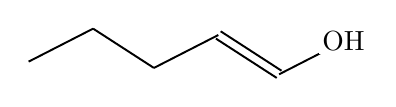
\begin{tikzpicture}[line width=.7pt]\draw (-2.000,-0.129)--(-1.181,0.290);
\draw (-1.181,0.290)--(-0.409,-0.209);
\draw (-0.409,-0.209)--(0.409,0.209);
\draw (0.379,0.163)--(1.151,-0.336);
\draw (0.439,0.256)--(1.211,-0.244);
\draw (1.181,-0.290)--(2.000,0.129);
\node[fill=white,inner sep=1.1pt]at(2.000,0.129){$\mathrm{OH}$};\end{tikzpicture}}\end{minipage}\begin{minipage}[c]{.48\linewidth}\centering (2)\par \scalebox{.83}{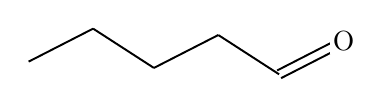
\begin{tikzpicture}[line width=.7pt]\draw (-2.000,-0.129)--(-1.181,0.290);
\draw (-1.181,0.290)--(-0.409,-0.209);
\draw (-0.409,-0.209)--(0.409,0.209);
\draw (0.409,0.209)--(1.181,-0.290);
\draw (1.206,-0.339)--(2.025,0.080);
\draw (1.156,-0.241)--(1.975,0.178);
\node[fill=white,inner sep=1.1pt]at(2.000,0.129){$\mathrm{O}$};\end{tikzpicture}}\end{minipage}\par\medskip\par\smallskip \textbf{推导：}末端炔烃为1-戊炔。硼氢化将B引到较少取代的末端碳，氧化以OH替B形成末端烯醇；再经酮—烯醇互变得到戊醛。互变只转移氢和$\pi$键，不改变碳骨架。\par\smallskip \par\smallskip \textbf{反校：}起料与两产物都是5C；空1为烯醇而非饱和醇；空2是端醛而非2-戊酮。\par\smallskip \par\smallskip \textbf{2分参考采分：}烯醇1分；戊醛1分。\par\smallskip \par\smallskip \textbf{边界/原印问题：}原B2H6符号保留；不补造选择性比例，按原题教材硼氢化氧化模型给主要结构。\par\smallskip \par\smallskip 独立推导后对照本书参考答案PDF111页；有原答案缺笔处以原题碳骨架/反应守恒校正，不盲抄。\par\smallskip \par\medskip\clearpage\subsection*{12．（2分）}原书：华东理工大学模拟试题（一） 一、回答问题 第27题；PDF[107]，印刷页[102]。\par\smallskip 完成反应，填写全部原空\par\smallskip \par\smallskip 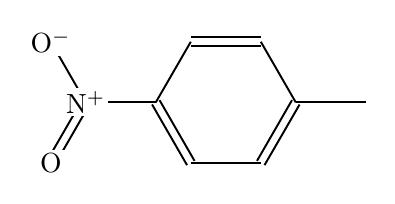
\begin{tikzpicture}[line width=.7pt]\draw (2.000,0.000)--(1.111,0.000);
\draw (1.111,0.000)--(0.667,0.770);
\draw (0.667,0.825)--(-0.222,0.825);
\draw (0.667,0.715)--(-0.222,0.715);
\draw (-0.222,0.770)--(-0.667,0.000);
\draw (-0.667,0.000)--(-1.556,0.000);
\draw (-1.603,0.028)--(-2.048,-0.742);
\draw (-1.508,-0.027)--(-1.952,-0.797);
\draw (-1.556,0.000)--(-2.000,0.770);
\draw (-0.714,-0.027)--(-0.270,-0.797);
\draw (-0.619,0.028)--(-0.175,-0.742);
\draw (-0.222,-0.770)--(0.667,-0.770);
\draw (0.714,-0.797)--(1.159,-0.028);
\draw (0.619,-0.742)--(1.063,0.028);
\node[fill=white,inner sep=1.1pt]at(-1.556,0.000){$\mathrm{N^{+}}$};
\node[fill=white,inner sep=1.1pt]at(-2.000,-0.770){$\mathrm{O}$};
\node[fill=white,inner sep=1.1pt]at(-2.000,0.770){$\mathrm{O^{-}}$};\end{tikzpicture}$\xrightarrow{\ Fe/HCl\ }$（空1）$\xrightarrow{\ NaNO_2,HCl;0\!\sim\!5^\circ C\ }$（空2）\par\smallskip 再与下列化合物在弱酸性条件下反应：\par\smallskip 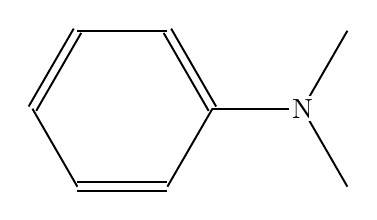
\begin{tikzpicture}[line width=.7pt]\draw (2.000,-0.990)--(1.429,0.000);
\draw (1.429,0.000)--(2.000,0.990);
\draw (1.429,0.000)--(0.286,0.000);
\draw (0.333,0.028)--(-0.238,1.017);
\draw (0.238,-0.027)--(-0.333,0.962);
\draw (-0.286,0.990)--(-1.429,0.990);
\draw (-1.476,1.017)--(-2.048,0.028);
\draw (-1.381,0.962)--(-1.952,-0.027);
\draw (-2.000,0.000)--(-1.429,-0.990);
\draw (-1.429,-1.045)--(-0.286,-1.045);
\draw (-1.429,-0.935)--(-0.286,-0.935);
\draw (-0.286,-0.990)--(0.286,0.000);
\node[fill=white,inner sep=1.1pt]at(1.429,0.000){$\mathrm{N}$};\end{tikzpicture}$\xrightarrow{\ \text{弱酸性}\ }$（空3）\par\smallskip \par\smallskip \textbf{答案（顺原空次序）：}\par\smallskip \begin{minipage}[c]{.32\linewidth}\centering (1)\par \scalebox{.83}{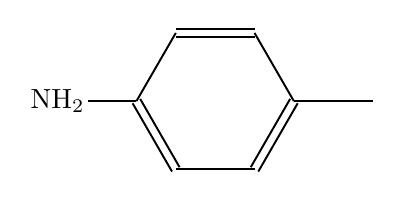
\begin{tikzpicture}[line width=.7pt]\draw (2.000,0.000)--(1.000,0.000);
\draw (1.000,0.000)--(0.500,0.866);
\draw (0.500,0.921)--(-0.500,0.921);
\draw (0.500,0.811)--(-0.500,0.811);
\draw (-0.500,0.866)--(-1.000,0.000);
\draw (-1.000,0.000)--(-2.000,0.000);
\draw (-1.048,-0.027)--(-0.548,-0.894);
\draw (-0.952,0.028)--(-0.452,-0.839);
\draw (-0.500,-0.866)--(0.500,-0.866);
\draw (0.548,-0.894)--(1.048,-0.027);
\draw (0.452,-0.839)--(0.952,0.028);
\node[fill=white,inner sep=1.1pt]at(-2.000,0.000){$\mathrm{NH_{2}}$};\end{tikzpicture}}\end{minipage}\begin{minipage}[c]{.32\linewidth}\centering (2)\par \scalebox{.83}{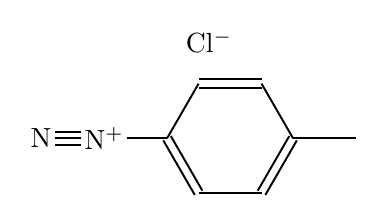
\begin{tikzpicture}[line width=.7pt]\draw (2.000,-0.267)--(1.200,-0.267);
\draw (1.200,-0.267)--(0.800,0.426);
\draw (0.800,0.481)--(0.000,0.481);
\draw (0.800,0.371)--(0.000,0.371);
\draw (0.000,0.426)--(-0.400,-0.267);
\draw (-0.400,-0.267)--(-1.200,-0.267);
\draw (-1.200,-0.184)--(-2.000,-0.184);
\draw (-1.200,-0.267)--(-2.000,-0.267);
\draw (-1.200,-0.349)--(-2.000,-0.349);
\draw (-0.448,-0.294)--(-0.048,-0.987);
\draw (-0.352,-0.239)--(0.048,-0.932);
\draw (-0.000,-0.959)--(0.800,-0.959);
\draw (0.848,-0.987)--(1.248,-0.294);
\draw (0.752,-0.932)--(1.152,-0.239);
\node[fill=white,inner sep=1.1pt]at(-1.200,-0.267){$\mathrm{N^{+}}$};
\node[fill=white,inner sep=1.1pt]at(-2.000,-0.267){$\mathrm{N}$};
\node[fill=white,inner sep=1.1pt]at(0.133,0.959){$\mathrm{Cl^{-}}$};\end{tikzpicture}}\end{minipage}\begin{minipage}[c]{.32\linewidth}\centering (3)\par \scalebox{.83}{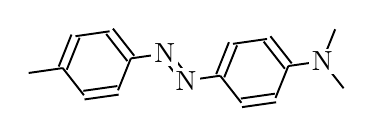
\begin{tikzpicture}[line width=.7pt]\draw (-2.000,-0.088)--(-1.567,-0.026);
\draw (-1.567,-0.026)--(-1.298,-0.370);
\draw (-1.290,-0.424)--(-0.857,-0.363);
\draw (-1.305,-0.315)--(-0.873,-0.254);
\draw (-0.865,-0.308)--(-0.702,0.097);
\draw (-0.702,0.097)--(-0.270,0.159);
\draw (-0.313,0.125)--(-0.043,-0.219);
\draw (-0.226,0.193)--(0.043,-0.151);
\draw (0.000,-0.185)--(0.433,-0.123);
\draw (0.433,-0.123)--(0.702,-0.467);
\draw (0.710,-0.522)--(1.143,-0.460);
\draw (0.695,-0.413)--(1.127,-0.351);
\draw (1.135,-0.405)--(1.298,0.000);
\draw (1.298,0.000)--(1.730,0.062);
\draw (1.730,0.062)--(2.000,-0.282);
\draw (1.730,0.062)--(1.893,0.467);
\draw (1.341,0.034)--(1.071,0.378);
\draw (1.254,-0.034)--(0.985,0.310);
\draw (1.028,0.344)--(0.595,0.282);
\draw (-0.659,0.131)--(-0.929,0.475);
\draw (-0.746,0.063)--(-1.015,0.407);
\draw (-0.972,0.441)--(-1.405,0.379);
\draw (-1.456,0.400)--(-1.618,-0.006);
\draw (-1.353,0.359)--(-1.516,-0.047);
\draw (0.544,0.303)--(0.382,-0.103);
\draw (0.647,0.262)--(0.484,-0.144);
\node[fill=white,inner sep=1.1pt]at(-0.270,0.159){$\mathrm{N}$};
\node[fill=white,inner sep=1.1pt]at(0.000,-0.185){$\mathrm{N}$};
\node[fill=white,inner sep=1.1pt]at(1.730,0.062){$\mathrm{N}$};\end{tikzpicture}}\end{minipage}\par\medskip\par\medskip\par\smallskip \textbf{推导：}Fe/HCl把NO2还原为NH2；低温亚硝酸使芳香伯胺重氮化，保留甲基与重氮基的对位关系。最后以N,N-二甲基苯胺富电子芳环的对位进攻重氮端氮，脱质子恢复芳香性，形成偶氮键。\par\smallskip \par\smallskip \textbf{反校：}两苯环之间必须是N=N，不能画成N—N单键；NMe2不被替换；对位尚空，不能优先给邻位唯一答案。\par\smallskip \par\smallskip \textbf{2分参考采分：}对甲苯胺0.5分；重氮盐0.5分；对位偶氮产物1分。\par\smallskip \par\smallskip \textbf{边界/原印问题：}还原步骤酸性介质中胺可质子化；接受后续重氮化前后相应酸碱形式，不改变骨架。\par\smallskip \par\smallskip 独立推导后对照本书参考答案PDF111页；有原答案缺笔处以原题碳骨架/反应守恒校正，不盲抄。\par\smallskip \par\medskip\clearpage\subsection*{13．（2分）}原书：华东理工大学模拟试题（一） 一、回答问题 第30题；PDF[107]，印刷页[102]。\par\smallskip 完成反应，填写全部原空\par\smallskip \par\smallskip 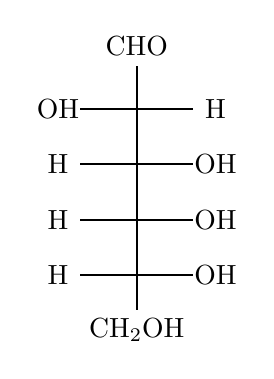
\begin{tikzpicture}[line width=.7pt]\node at(0,2.8){$\mathrm{CHO}$};
\draw(0,2.55)--(0,-.55);
\node at(0,-.8){$\mathrm{CH_2OH}$};
\draw(-.72,2)--(.72,2);
\node at(-1.0,2){$\mathrm{OH}$};
\node at(1.0,2){$\mathrm{H}$};
\draw(-.72,1.3)--(.72,1.3);
\node at(-1.0,1.3){$\mathrm{H}$};
\node at(1.0,1.3){$\mathrm{OH}$};
\draw(-.72,0.6)--(.72,0.6);
\node at(-1.0,0.6){$\mathrm{H}$};
\node at(1.0,0.6){$\mathrm{OH}$};
\draw(-.72,-0.1)--(.72,-0.1);
\node at(-1.0,-0.1){$\mathrm{H}$};
\node at(1.0,-0.1){$\mathrm{OH}$};\end{tikzpicture}$\xrightarrow{\ 3C_6H_5NHNH_2\ }$（空）\par\smallskip \par\smallskip \textbf{答案（顺原空次序）：}\par\smallskip 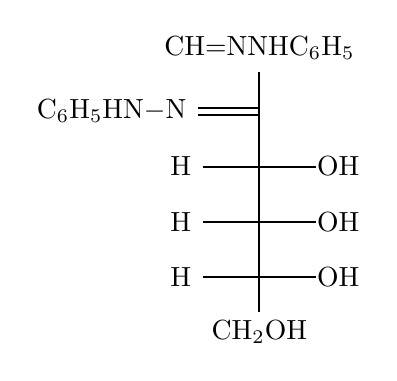
\begin{tikzpicture}[line width=.7pt]\node at(0,2.8){$\mathrm{CH{=}NNHC_6H_5}$};
\draw(0,2.5)--(0,-.55);
\node at(0,-.8){$\mathrm{CH_2OH}$};
\draw(0,2.04)--(-.78,2.04);\draw(0,1.96)--(-.78,1.96);
\node[anchor=east]at(-.8,2){$\mathrm{C_6H_5HN{-}N}$};
\draw(-.72,1.3)--(.72,1.3);
\node at(-1.,1.3){$\mathrm{H}$};
\node at(1.,1.3){$\mathrm{OH}$};
\draw(-.72,0.6)--(.72,0.6);
\node at(-1.,0.6){$\mathrm{H}$};
\node at(1.,0.6){$\mathrm{OH}$};
\draw(-.72,-0.1)--(.72,-0.1);
\node at(-1.,-0.1){$\mathrm{H}$};
\node at(1.,-0.1){$\mathrm{OH}$};\end{tikzpicture}\par\smallskip \textbf{推导：}此Fischer式C2羟基向左，C3、C4、C5均向右。糖脎形成会把C1醛基和相邻C2醇碳都转为苯腙单元；C3—C5不参与氧化，原羟基方向全部保留。三当量苯肼中两当量留在糖脎，一当量承担氧化所需的转化并形成苯胺与氨。\par\smallskip \par\smallskip \textbf{反校：}C1为CH=NNHPh；C2为C(=NNHPh)，不再有H/OH；C3—C5的OH仍全在右；不是只作单苯腙。\par\smallskip \par\smallskip \textbf{2分参考采分：}C1/C2双苯腙1分；C3—C5及CH2OH正确保留1分。\par\smallskip \par\smallskip 独立推导后对照本书参考答案PDF111页；有原答案缺笔处以原题碳骨架/反应守恒校正，不盲抄。\par\smallskip \par\medskip\clearpage\subsection*{14．（2分）}原书：复旦大学模拟试题（三） 二、完成反应 第10题；PDF[156]，印刷页[151]。\par\smallskip 完成反应，填写全部原空\par\smallskip \par\smallskip 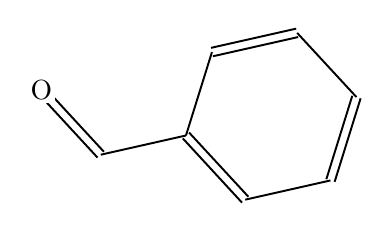
\begin{tikzpicture}[line width=.7pt]\draw (-2.040,0.290)--(-1.288,-0.525);
\draw (-1.960,0.365)--(-1.207,-0.451);
\draw (-1.247,-0.488)--(-0.165,-0.244);
\draw (-0.205,-0.281)--(0.547,-1.097);
\draw (-0.125,-0.207)--(0.628,-1.022);
\draw (0.588,-1.059)--(1.670,-0.815);
\draw (1.723,-0.832)--(2.053,0.228);
\draw (1.618,-0.799)--(1.947,0.260);
\draw (2.000,0.244)--(1.247,1.059);
\draw (1.235,1.113)--(0.153,0.869);
\draw (1.259,1.006)--(0.177,0.762);
\draw (0.165,0.815)--(-0.165,-0.244);
\node[fill=white,inner sep=1.1pt]at(-2.000,0.327){$\mathrm{O}$};\end{tikzpicture}$+\mathrm{MeNH_2}$$\xrightarrow{\ NaBH_3(CN)\ }$（空）\par\smallskip \par\smallskip \textbf{答案（顺原空次序）：}\par\smallskip \par\medskip 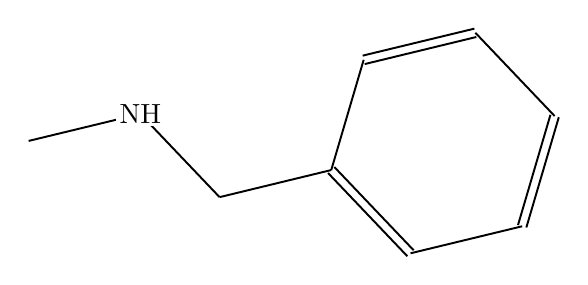
\begin{tikzpicture}[line width=.7pt]\draw (-3.340,0.027)--(-1.922,0.370);
\draw (-1.922,0.370)--(-0.915,-0.687);
\draw (-0.915,-0.687)--(0.503,-0.343);
\draw (0.463,-0.381)--(1.470,-1.438);
\draw (0.543,-0.305)--(1.550,-1.362);
\draw (1.510,-1.400)--(2.928,-1.057);
\draw (2.981,-1.072)--(3.393,0.328);
\draw (2.875,-1.041)--(3.287,0.359);
\draw (3.340,0.343)--(2.334,1.400);
\draw (2.321,1.453)--(0.902,1.110);
\draw (2.346,1.347)--(0.928,1.003);
\draw (0.915,1.057)--(0.503,-0.343);
\node[fill=white,inner sep=1.1pt]at(-1.922,0.370){$\mathrm{NH}$};\end{tikzpicture}\par\medskip\par\smallskip \textbf{推导：}苯甲醛与甲胺先经亲核加成、脱水形成亚胺/亚胺正离子中间体，氰基硼氢化物将C=N还原成C—N。醛碳成为苄基CH2，原甲胺的甲基仍连在N上，得到N-甲基苄胺。\par\smallskip \par\smallskip \textbf{反校：}碳数6+1+1=8；产物是仲胺NH，不能画成N,N-二甲基胺，也不能停在亚胺。\par\smallskip \par\smallskip \textbf{2分参考采分：}PhCH2—N连接1分；N上甲基及一个H正确1分。\par\smallskip \par\smallskip \textbf{边界/原印问题：}原印NaBH3(CN)原样保留，按NaBH3CN的括写识别，不擅换NaBH4。\par\smallskip \par\smallskip 独立推导后对照本书参考答案PDF158页；有原答案缺笔处以原题碳骨架/反应守恒校正，不盲抄。\par\smallskip \par\medskip\clearpage\subsection*{15．（2分）}原书：复旦大学模拟试题（三） 二、完成反应 第11题；PDF[156]，印刷页[151]。\par\smallskip 完成反应，填写全部原空\par\smallskip \par\smallskip 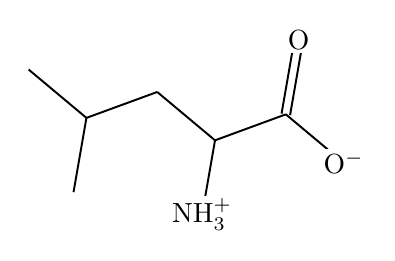
\begin{tikzpicture}[line width=.7pt]\draw (-2.000,0.734)--(-1.266,0.120);
\draw (-1.266,0.120)--(-1.430,-0.823);
\draw (-1.266,0.120)--(-0.367,0.449);
\draw (-0.367,0.449)--(0.367,-0.165);
\draw (0.367,-0.165)--(0.203,-1.107);
\draw (0.367,-0.165)--(1.266,0.165);
\draw (1.320,0.155)--(1.484,1.098);
\draw (1.212,0.174)--(1.376,1.117);
\draw (1.266,0.165)--(2.000,-0.449);
\node[fill=white,inner sep=1.1pt]at(0.203,-1.107){$\mathrm{NH_{3}^{+}}$};
\node[fill=white,inner sep=1.1pt]at(1.430,1.107){$\mathrm{O}$};
\node[fill=white,inner sep=1.1pt]at(2.000,-0.449){$\mathrm{O^{-}}$};\end{tikzpicture}$+$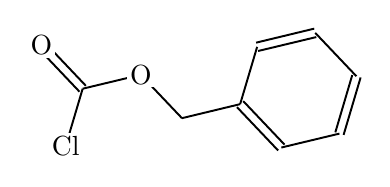
\begin{tikzpicture}[line width=.7pt]\draw (-2.040,0.532)--(-1.517,-0.019);
\draw (-1.960,0.608)--(-1.437,0.057);
\draw (-1.477,0.019)--(-1.693,-0.709);
\draw (-1.477,0.019)--(-0.739,0.196);
\draw (-0.739,0.196)--(-0.216,-0.355);
\draw (-0.216,-0.355)--(0.523,-0.177);
\draw (0.483,-0.215)--(1.006,-0.766);
\draw (0.563,-0.139)--(1.086,-0.690);
\draw (1.046,-0.728)--(1.784,-0.551);
\draw (1.837,-0.567)--(2.053,0.162);
\draw (1.732,-0.535)--(1.947,0.193);
\draw (2.000,0.177)--(1.477,0.728);
\draw (1.464,0.782)--(0.726,0.604);
\draw (1.490,0.675)--(0.751,0.498);
\draw (0.739,0.551)--(0.523,-0.177);
\node[fill=white,inner sep=1.1pt]at(-2.000,0.570){$\mathrm{O}$};
\node[fill=white,inner sep=1.1pt]at(-1.693,-0.709){$\mathrm{Cl}$};
\node[fill=white,inner sep=1.1pt]at(-0.739,0.196){$\mathrm{O}$};\end{tikzpicture}$\xrightarrow{\ \ }$（空）\par\smallskip \par\smallskip \textbf{答案（顺原空次序）：}\par\smallskip \par\medskip 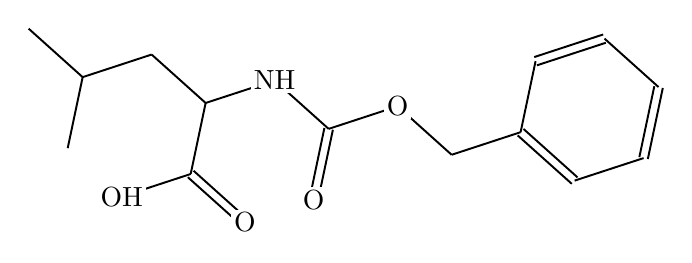
\begin{tikzpicture}[line width=.7pt]\draw (-4.000,1.231)--(-3.314,0.615);
\draw (-3.314,0.615)--(-3.504,-0.287);
\draw (-3.314,0.615)--(-2.438,0.902);
\draw (-2.438,0.902)--(-1.752,0.287);
\draw (-1.752,0.287)--(-0.876,0.573);
\draw (-0.876,0.573)--(-0.190,-0.042);
\draw (-0.244,-0.031)--(-0.433,-0.933);
\draw (-0.136,-0.053)--(-0.326,-0.955);
\draw (-0.190,-0.042)--(0.686,0.245);
\draw (0.686,0.245)--(1.372,-0.371);
\draw (1.372,-0.371)--(2.248,-0.084);
\draw (2.211,-0.125)--(2.898,-0.740);
\draw (2.285,-0.043)--(2.971,-0.658);
\draw (2.934,-0.699)--(3.810,-0.413);
\draw (3.864,-0.424)--(4.054,0.478);
\draw (3.756,-0.401)--(3.946,0.500);
\draw (4.000,0.489)--(3.314,1.104);
\draw (3.297,1.157)--(2.421,0.870);
\draw (3.331,1.052)--(2.455,0.765);
\draw (-1.752,0.287)--(-1.942,-0.615);
\draw (-1.978,-0.656)--(-1.292,-1.271);
\draw (-1.905,-0.574)--(-1.219,-1.190);
\draw (-1.942,-0.615)--(-2.817,-0.902);
\draw (2.438,0.818)--(2.248,-0.084);
\node[fill=white,inner sep=1.1pt]at(-0.876,0.573){$\mathrm{NH}$};
\node[fill=white,inner sep=1.1pt]at(-0.380,-0.944){$\mathrm{O}$};
\node[fill=white,inner sep=1.1pt]at(0.686,0.245){$\mathrm{O}$};
\node[fill=white,inner sep=1.1pt]at(-1.255,-1.231){$\mathrm{O}$};
\node[fill=white,inner sep=1.1pt]at(-2.817,-0.902){$\mathrm{OH}$};\end{tikzpicture}\par\medskip\par\smallskip \textbf{推导：}起料是亮氨酸两性离子，侧链必须保留CH2CH(CH3)2。氨基对氯甲酸苄酯羰基取代，生成N-Cbz氨基甲酸酯，保护基连接顺序为N—C(=O)—O—CH2Ph。按教材后处理表达为游离羧酸；这不是羧基苄酯化。\par\smallskip \par\smallskip \textbf{反校：}保留异丁基支链；仅N引入一个Cbz；原图没有楔虚线，不能凭空指定L/D或R/S。\par\smallskip \par\smallskip \textbf{2分参考采分：}N-Cbz正确连接1分；原侧链和羧酸正确1分。\par\smallskip \par\smallskip \textbf{边界/原印问题：}原图未给绝对构型，题源粗筛所谓“必有手性信息”现纠正为未指定；原箭头未印碱/后处理，说明常规N保护模型，不虚称定量反应。本书参考答案此处侧链印得不完整；本答案依据原题真实亮氨酸支链保留，不能照错图删碳。\par\smallskip \par\smallskip 独立推导后对照本书参考答案PDF158页；有原答案缺笔处以原题碳骨架/反应守恒校正，不盲抄。\par\smallskip \par\medskip\clearpage\clearpage\section*{二、选择题（12题，共12分）}\subsection*{1．（1分）}\textbf{参考答案：A}\par\medskip{}\subsection*{独立推导}
\par 先选择最高顺序特征基团：羧酸优先于羟基，母体用苯甲酸。与羧基连接的环碳为1号，不把羧基碳算进苯环编号。
\par 从靠近甲基的一侧编号，甲基在3位，羟基在4位，另一方向会给甲基5位，不取。故为4-羟基-3-甲基苯甲酸。
\subsection*{各选项依据}
\par\textbf{A：}选用苯甲酸母体，3-甲基与4-羟基均和结构一致。
\par\textbf{B：}把酚当母体而把羧酸作低顺序前缀，不符合本题IUPAC系统命名要求。
\par\textbf{C：}把甲苯当母体，同样没有用最高顺序羧酸作主要官能团。
\par\textbf{D：}混用对/间位置词，不是本题所求以数字定位的规范系统名。
\subsection*{第三轮反校}
\par 从名称A反画：环1接COOH、3接Me、4接OH，逐项与原图吻合。
\par 只改变画图朝向不改变3/4定位；未擅自把末端甲基改作额外主链碳。
\par\medskip\clearpage\subsection*{2．（1分）}\textbf{参考答案：3}\par\medskip{}原书1.3同步练习2；印21页/PDF26页。\par 下列化合物中沸点最低的是：\par\medskip
\begin{minipage}[c][3.4cm][c]{.48\linewidth}\centering (1)\par\smallskip \scalebox{.73}{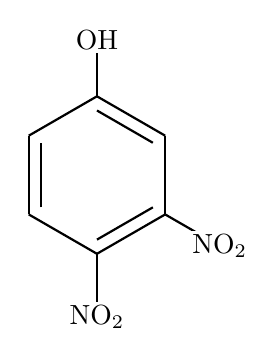
\begin{tikzpicture}[line width=.8pt]\draw (0.000,1.000)--(0.866,0.500);
\draw (0.000,0.820)--(0.710,0.410);
\draw (0.866,0.500)--(0.866,-0.500);
\draw (0.866,-0.500)--(0.000,-1.000);
\draw (0.710,-0.410)--(0.000,-0.820);
\draw (0.000,-1.000)--(-0.866,-0.500);
\draw (-0.866,-0.500)--(-0.866,0.500);
\draw (-0.710,-0.410)--(-0.710,0.410);
\draw (-0.866,0.500)--(0.000,1.000);
\draw (0.000,1.000)--(0.000,1.580);
\node[fill=white,inner sep=1.1pt] at (0.000,1.713) {$\mathrm{OH}$};
\draw (0.866,-0.500)--(1.429,-0.825);
\node[fill=white,inner sep=1.1pt] at (1.558,-0.900) {$\mathrm{NO_2}$};
\draw (0.000,-1.000)--(0.000,-1.650);
\node[fill=white,inner sep=1.1pt] at (0.000,-1.799) {$\mathrm{NO_2}$};\end{tikzpicture}}\end{minipage}\hfill
\begin{minipage}[c][3.4cm][c]{.48\linewidth}\centering (2)\par\smallskip \scalebox{.73}{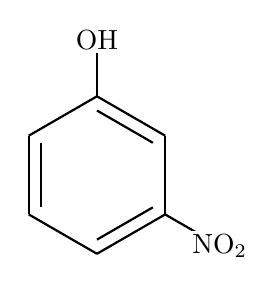
\begin{tikzpicture}[line width=.8pt]\draw (0.000,1.000)--(0.866,0.500);
\draw (0.000,0.820)--(0.710,0.410);
\draw (0.866,0.500)--(0.866,-0.500);
\draw (0.866,-0.500)--(0.000,-1.000);
\draw (0.710,-0.410)--(0.000,-0.820);
\draw (0.000,-1.000)--(-0.866,-0.500);
\draw (-0.866,-0.500)--(-0.866,0.500);
\draw (-0.710,-0.410)--(-0.710,0.410);
\draw (-0.866,0.500)--(0.000,1.000);
\draw (0.000,1.000)--(0.000,1.580);
\node[fill=white,inner sep=1.1pt] at (0.000,1.713) {$\mathrm{OH}$};
\draw (0.866,-0.500)--(1.429,-0.825);
\node[fill=white,inner sep=1.1pt] at (1.558,-0.900) {$\mathrm{NO_2}$};\end{tikzpicture}}\end{minipage}\par
\begin{minipage}[c][3.4cm][c]{.48\linewidth}\centering (3)\par\smallskip \scalebox{.73}{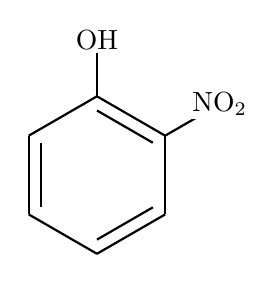
\begin{tikzpicture}[line width=.8pt]\draw (0.000,1.000)--(0.866,0.500);
\draw (0.000,0.820)--(0.710,0.410);
\draw (0.866,0.500)--(0.866,-0.500);
\draw (0.866,-0.500)--(0.000,-1.000);
\draw (0.710,-0.410)--(0.000,-0.820);
\draw (0.000,-1.000)--(-0.866,-0.500);
\draw (-0.866,-0.500)--(-0.866,0.500);
\draw (-0.710,-0.410)--(-0.710,0.410);
\draw (-0.866,0.500)--(0.000,1.000);
\draw (0.000,1.000)--(0.000,1.580);
\node[fill=white,inner sep=1.1pt] at (0.000,1.713) {$\mathrm{OH}$};
\draw (0.866,0.500)--(1.429,0.825);
\node[fill=white,inner sep=1.1pt] at (1.558,0.900) {$\mathrm{NO_2}$};\end{tikzpicture}}\end{minipage}\hfill
\begin{minipage}[c][3.4cm][c]{.48\linewidth}\centering (4)\par\smallskip \scalebox{.73}{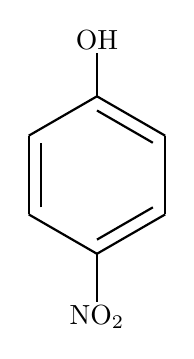
\begin{tikzpicture}[line width=.8pt]\draw (0.000,1.000)--(0.866,0.500);
\draw (0.000,0.820)--(0.710,0.410);
\draw (0.866,0.500)--(0.866,-0.500);
\draw (0.866,-0.500)--(0.000,-1.000);
\draw (0.710,-0.410)--(0.000,-0.820);
\draw (0.000,-1.000)--(-0.866,-0.500);
\draw (-0.866,-0.500)--(-0.866,0.500);
\draw (-0.710,-0.410)--(-0.710,0.410);
\draw (-0.866,0.500)--(0.000,1.000);
\draw (0.000,1.000)--(0.000,1.580);
\node[fill=white,inner sep=1.1pt] at (0.000,1.713) {$\mathrm{OH}$};
\draw (0.000,-1.000)--(0.000,-1.650);
\node[fill=white,inner sep=1.1pt] at (0.000,-1.799) {$\mathrm{NO_2}$};\end{tikzpicture}}\end{minipage}\par
\textbf{答案：}(3)。\par\textbf{从基础到判断：}沸腾需克服分子之间的吸引力，而不是打断分子内共价键。先识别四项都是含酚羟基的芳香化合物，再检查是否能形成分子内氢键。邻位硝基与羟基相邻，使羟基供氢、硝基氧受氢形成分子内氢键，减少分子间缔合，因此本题选(3)。\par\textbf{逐项核验：}\begin{enumerate}
\item 两个硝基，未形成(3)那种邻位羟基—硝基内氢键，不能因硝基多就判最低。
\item 硝基在间位，不能形成邻位六元内氢键。
\item 邻硝基苯酚：分子内氢键使分子间缔合作用减弱，为最低项。
\item 对硝基苯酚仍能形成明显分子间氢键，不选。
\end{enumerate}\textbf{易错与边界：}内氢键并非使一切物性都降低；此处是在相同外压、同系列中判断沸点。不要把“熔点高低”与沸点规则混用。\par\smallskip 第三轮：复核否定词、原标签、逐项连接/电荷与完整共轭；独立判断后对照原书参考答案（PDF244页）一致。\par\medskip\clearpage\subsection*{3．（1分）}\textbf{参考答案：A}\par\medskip{}模拟试题1·一·1\quad 印刷115页 / PDF 124页
\par\bigskip
下列哪种烯烃的氢化热最小？（\quad）
\par\bigskip
\begin{minipage}[t]{.48\linewidth}\vspace{0pt}\textbf{(A)}\par\smallskip $E$-2-丁烯\end{minipage}\hfill
\begin{minipage}[t]{.48\linewidth}\vspace{0pt}\textbf{(B)}\par\smallskip $Z$-2-丁烯\end{minipage}\par\bigskip
\begin{minipage}[t]{.48\linewidth}\vspace{0pt}\textbf{(C)}\par\smallskip 1-丁烯\end{minipage}\hfill
\begin{minipage}[t]{.48\linewidth}\vspace{0pt}\textbf{(D)}\par\smallskip 异丁烯\end{minipage}\par\bigskip
\par\bigskip\textbf{教师答案：}A
\par\medskip\textbf{从依据到结论：}先识别氢化热为加氢放热量的大小。相同碳数烯烃中，内部双键和反式排列通常降低烯烃能量；反式2-丁烯的加氢放热量在这四项中最小。
\par\medskip\textbf{选项排除：}B为顺式，两个甲基较靠近；C为端烯；D为偕二取代烯烃，不能只凭支链较多就选D。
\par\medskip\textbf{反向核对及边界：}不把放热量最小误写为带负号焓变数值最小；不同氢化产物的比较不能无限推广。
\par\smallskip 本书对照：印刷118页，原答案A。
\par\medskip\clearpage\subsection*{4．（1分）}\textbf{参考答案：D}\par\medskip{}模拟试题4·一·1\quad 印刷134页 / PDF 143页
\par\bigskip
化合物：\par\medskip\noindent \(\mathrm{I:\ CH_3CH_2CH(Cl)COO^-}\)\quad \(\mathrm{II:\ CH_3CH_2C(Cl)_2COO^-}\)\par\medskip \(\mathrm{III:\ CH_3CH_2CH(CH_3)COO^-}\)\quad \(\mathrm{IV:\ CH_3CH_2CH_2COO^-}\)\par\medskip 碱性强弱次序是（\quad）。
\par\bigskip
\begin{minipage}[t]{.48\linewidth}\vspace{0pt}\textbf{(A)}\par\smallskip $\mathrm{I>II>III>IV}$\end{minipage}\hfill
\begin{minipage}[t]{.48\linewidth}\vspace{0pt}\textbf{(B)}\par\smallskip $\mathrm{II>III>I>IV}$\end{minipage}\par\bigskip
\begin{minipage}[t]{.48\linewidth}\vspace{0pt}\textbf{(C)}\par\smallskip $\mathrm{III>II>I>IV}$\end{minipage}\hfill
\begin{minipage}[t]{.48\linewidth}\vspace{0pt}\textbf{(D)}\par\smallskip $\mathrm{III>IV>I>II}$\end{minipage}\par\bigskip
\par\bigskip\textbf{教师答案：}D
\par\medskip\textbf{从依据到结论：}先看各项均为羧酸根，比较取代基对负离子的稳定作用。氯的吸电子诱导效应使负离子更稳定、碱性更弱；两个氯的作用大于一个氯。烷基给电子使III较IV碱性增强，得到III>IV>I>II。
\par\medskip\textbf{选项排除：}A把氯代与烷基给电子关系颠倒；B和C把二氯项排得太强。
\par\medskip\textbf{反向核对及边界：}比较的是羧酸根碱性，若改比较对应羧酸酸性，顺序反向。
\par\smallskip 本书对照：印刷137页，原答案D。
\par\medskip\clearpage\subsection*{5．（1分）}\textbf{参考答案：A}\par\medskip{}\subsection*{独立推导}
\par 比较碱性要考查接受质子的能力，通常可借共轭酸稳定性理解；不能把含NH的酸性当作碱性。
\par 氨的孤对没有和芳环或羰基离域；苯胺的孤对与苯环共轭，作碱的能力下降。酰胺孤对与羰基强烈离域，使氮极弱碱；磺酰胺受到SO2基更强的吸电子/离域影响，课程模型下更弱。得到a>b>c>d。
\subsection*{各选项依据}
\par\textbf{A：}与氨、芳胺、酰胺、磺酰胺的常规分类顺序相符。
\par\textbf{B：}把最弱的磺酰胺放在最强一端，方向相反。
\par\textbf{C：}把苯胺放在氨之前，忽略芳环对氮孤对的离域。
\par\textbf{D：}同时把磺酰胺置顶、酰胺强于苯胺，均不成立。
\subsection*{第三轮反校}
\par 单独核前两者：氨共轭酸pKa约9.26，苯胺约4.63，故a>b；这些只是已核教材辅助值，不给后两者杜撰精确pKa。
\par 强酸中酰胺可能优先在O上质子化，因此解析不把“酰胺完全永不受质子”当普适断言。
\subsection*{适用边界}
按通常稀溶液课程分类比较；原题没有给可外推到任意超强酸/气相的实验全序。
\par 核对入口：\url{https://openstax.org/books/organic-chemistry/pages/24-3-basicity-of-amines}
\par\medskip\clearpage\subsection*{6．（1分）}\textbf{参考答案：D}\par\medskip{}\subsection*{独立推导}
\par SN2要求亲核体沿离去基团的背面进攻，使成键与断键在同一步发生；先判断带Br碳是否为可接近的sp3碳。
\par D的Br接在一级苄基CH2上，背面位阻小，苄位还能稳定SN2过渡态。A是芳基，C是乙烯基，均不按普通饱和碳SN2途径快速反应；B是刚性桥头，背面进攻受骨架限制。
\subsection*{各选项依据}
\par\textbf{A：}Br直接连芳环sp2碳，不是苄基溴。
\par\textbf{B：}Br在桥头，不能把整个桥环仅看成一个普通烷基。
\par\textbf{C：}Br直接连烯碳，普通SN2受阻，不能把烯丙位和乙烯基混淆。
\par\textbf{D：}一级苄基溴具备普通SN2有利条件。
\subsection*{第三轮反校}
\par 逐图核Br所连碳：A芳碳、B桥头碳、C烯碳、D苄基sp3碳；没有把D多删一个CH2。
\par 未把特殊苯炔/催化偶联条件混入题目未给的普通SN2比较。
\par\medskip\clearpage\subsection*{7．（1分）}\textbf{参考答案：C}\par\medskip{}\subsection*{独立推导}
\par 不要只看到有正负电试剂就判断机理，分别识别碳正离子、碳负离子、自由基和协同反应。
\par C中二苯甲基溴在水中溶剂解，可先离解形成由两个苯环稳定的二苯甲基碳正离子，再由水进攻和去质子得到醇。
\subsection*{各选项依据}
\par\textbf{A：}OH-催化乙醛羟醛加成，先形成烯醇负离子/烯醇盐，不需碳正离子。
\par\textbf{B：}光照氯代为自由基链过程，不以乙基碳正离子作传播中间体。
\par\textbf{C：}二苯甲基碳正离子可被两个苯环稳定，符合SN1溶剂解。
\par\textbf{D：}原图是Diels-Alder反应，通常按协同六电子环加成，不必生成自由碳正离子。
\subsection*{第三轮反校}
\par 用电荷回代C：C-Br异裂给正碳和Br-，水进攻后先为氧正离子，再去H+；得到原式的醇和HBr。
\par D照原六元共轭二烯/酸酐重绘，未替换成环戊二烯；笼状产物总C数10与6+4相同。
\par\medskip\clearpage\subsection*{8．（1分）}\textbf{参考答案：2、3、4}\par\medskip{}原书1.6同步练习1；印37页/PDF42页。\par 下列化合物或离子有芳香性的是：\par\medskip
\begin{minipage}[c][3.4cm][c]{.48\linewidth}\centering (1)\par\smallskip \scalebox{.73}{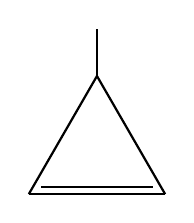
\begin{tikzpicture}[line width=.8pt]\draw (0.000,1.000)--(0.866,-0.500);
\draw (0.866,-0.500)--(-0.866,-0.500);
\draw (0.710,-0.410)--(-0.710,-0.410);
\draw (-0.866,-0.500)--(0.000,1.000);
\draw (0.000,1.000)--(0.000,1.600);\end{tikzpicture}}\end{minipage}\hfill
\begin{minipage}[c][3.4cm][c]{.48\linewidth}\centering (2)\par\smallskip \scalebox{.73}{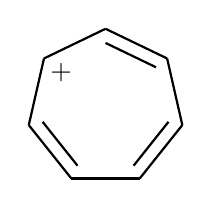
\begin{tikzpicture}[line width=.8pt]\draw (0.000,1.000)--(0.782,0.623);
\draw (0.000,0.820)--(0.641,0.511);
\draw (0.782,0.623)--(0.975,-0.223);
\draw (0.975,-0.223)--(0.434,-0.901);
\draw (0.799,-0.182)--(0.356,-0.739);
\draw (0.434,-0.901)--(-0.434,-0.901);
\draw (-0.434,-0.901)--(-0.975,-0.223);
\draw (-0.356,-0.739)--(-0.799,-0.182);
\draw (-0.975,-0.223)--(-0.782,0.623);
\draw (-0.782,0.623)--(0.000,1.000);
\node[fill=white,inner sep=1.1pt] at (-0.563,0.449) {$\mathrm{+}$};\end{tikzpicture}}\end{minipage}\par
\begin{minipage}[c][3.4cm][c]{.48\linewidth}\centering (3)\par\smallskip \scalebox{.73}{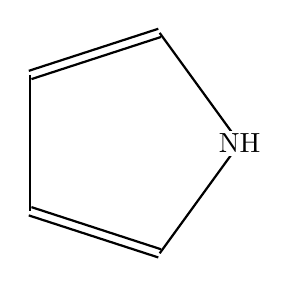
\begin{tikzpicture}[line width=.8pt]\draw (1.331,0.000)--(0.314,1.400);
\draw (0.297,1.452)--(-1.348,0.918);
\draw (0.331,1.348)--(-1.314,0.813);
\draw (-1.331,0.865)--(-1.331,-0.865);
\draw (-1.348,-0.918)--(0.297,-1.452);
\draw (-1.314,-0.813)--(0.331,-1.348);
\draw (0.314,-1.400)--(1.331,0.000);
\node[fill=white,inner sep=1.1pt]at(1.331,0.000){$\mathrm{NH}$};\end{tikzpicture}}\end{minipage}\hfill
\begin{minipage}[c][3.4cm][c]{.48\linewidth}\centering (4)\par\smallskip \scalebox{.73}{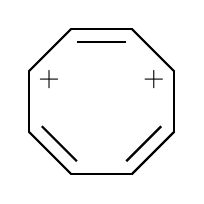
\begin{tikzpicture}[line width=.8pt]\draw (-0.383,0.924)--(0.383,0.924);
\draw (-0.314,0.758)--(0.314,0.758);
\draw (0.383,0.924)--(0.924,0.383);
\draw (0.924,0.383)--(0.924,-0.383);
\draw (0.924,-0.383)--(0.383,-0.924);
\draw (0.758,-0.314)--(0.314,-0.758);
\draw (0.383,-0.924)--(-0.383,-0.924);
\draw (-0.383,-0.924)--(-0.924,-0.383);
\draw (-0.314,-0.758)--(-0.758,-0.314);
\draw (-0.924,-0.383)--(-0.924,0.383);
\draw (-0.924,0.383)--(-0.383,0.924);
\node[fill=white,inner sep=1.1pt] at (0.665,0.276) {$\mathrm{+}$};
\node[fill=white,inner sep=1.1pt] at (-0.665,0.276) {$\mathrm{+}$};\end{tikzpicture}}\end{minipage}\par
\textbf{答案：}(2),(3),(4)。\par\textbf{从基础到判断：}芳香性先要求环状连续共轭和可有效重叠的p轨道，再按闭壳层Hückel模型检查4n+2个\(\pi\)电子。正电荷的空p轨道能参与共轭，却不给电子；吡咯氮的一对孤电子参与\(\pi\)系统。原题答案为(2)(3)(4)，明确为多项成立。\par\textbf{逐项核验：}\begin{enumerate}
\item 甲基取代的环丙烯，顶部是甲基短键而非正电荷；环上饱和碳中断共轭，不选。
\item 环庚三烯正离子：三条双键共6\(\pi\)电子，空p轨道补全环形共轭，选。
\item 吡咯：两条双键4电子，加N的一对孤电子2电子，合计6，选。
\item 环辛三烯二正离子：三条双键供6电子，两个带正电碳具有空p轨道，在所画闭壳层共轭结构中满足6\(\pi\)，选。
\end{enumerate}\textbf{易错与边界：}不能把(4)看作中性环辛四烯，也不能给每个正电荷额外加一电子。本题为所示结构的基础电子模型，不推断其溶液寿命。\par\smallskip 第三轮：复核否定词、原标签、逐项连接/电荷与完整共轭；独立判断后对照原书参考答案（PDF245页）一致。\par\medskip\clearpage\subsection*{9．（1分）}\textbf{参考答案：1、2}\par\medskip{}原书1.6同步练习4；印37页/PDF42页。\par 下列化合物有芳香性的是：\par\medskip
\begin{minipage}[c][3.4cm][c]{.48\linewidth}\centering (1)\par\smallskip \scalebox{.73}{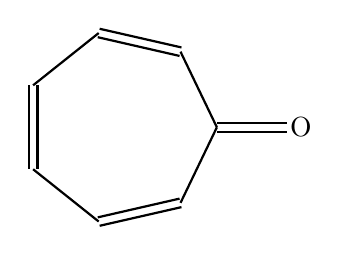
\begin{tikzpicture}[line width=.8pt]\draw (1.700,0.055)--(0.634,0.055);
\draw (1.700,-0.055)--(0.634,-0.055);
\draw (0.634,-0.000)--(0.172,0.960);
\draw (0.184,1.014)--(-0.855,1.251);
\draw (0.160,0.906)--(-0.879,1.144);
\draw (-0.867,1.197)--(-1.700,0.533);
\draw (-1.755,0.533)--(-1.755,-0.533);
\draw (-1.645,0.533)--(-1.645,-0.533);
\draw (-1.700,-0.533)--(-0.867,-1.197);
\draw (-0.855,-1.251)--(0.184,-1.014);
\draw (-0.879,-1.144)--(0.160,-0.906);
\draw (0.172,-0.960)--(0.634,-0.000);
\node[fill=white,inner sep=1.1pt]at(1.700,-0.000){$\mathrm{O}$};\end{tikzpicture}}\end{minipage}\hfill
\begin{minipage}[c][3.4cm][c]{.48\linewidth}\centering (2)\par\smallskip \scalebox{.73}{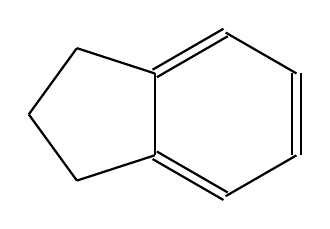
\begin{tikzpicture}[line width=.8pt]\draw (1.755,-0.520)--(1.755,0.520);
\draw (1.645,-0.520)--(1.645,0.520);
\draw (1.700,0.520)--(0.800,1.039);
\draw (0.772,1.087)--(-0.128,0.567);
\draw (0.827,0.992)--(-0.073,0.472);
\draw (-0.100,0.520)--(-0.100,-0.520);
\draw (-0.128,-0.567)--(0.772,-1.087);
\draw (-0.073,-0.472)--(0.827,-0.992);
\draw (-0.100,-0.520)--(-1.089,-0.841);
\draw (-1.089,-0.841)--(-1.700,0.000);
\draw (-1.700,0.000)--(-1.089,0.841);
\draw (0.800,-1.039)--(1.700,-0.520);
\draw (-1.089,0.841)--(-0.100,0.520);\end{tikzpicture}}\end{minipage}\par
\begin{minipage}[c][3.4cm][c]{.48\linewidth}\centering (3)\par\smallskip \scalebox{.73}{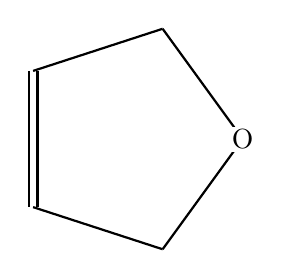
\begin{tikzpicture}[line width=.8pt]\draw (1.331,0.000)--(0.314,1.400);
\draw (0.314,1.400)--(-1.331,0.865);
\draw (-1.386,0.865)--(-1.386,-0.865);
\draw (-1.276,0.865)--(-1.276,-0.865);
\draw (-1.331,-0.865)--(0.314,-1.400);
\draw (0.314,-1.400)--(1.331,0.000);
\node[fill=white,inner sep=1.1pt]at(1.331,0.000){$\mathrm{O}$};\end{tikzpicture}}\end{minipage}\hfill
\begin{minipage}[c][3.4cm][c]{.48\linewidth}\centering (4)\par\smallskip \scalebox{.73}{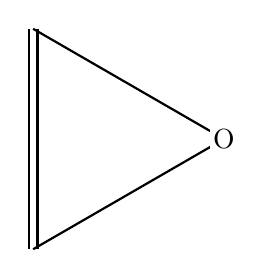
\begin{tikzpicture}[line width=.8pt]\draw (1.212,-0.000)--(-1.212,1.400);
\draw (-1.267,1.400)--(-1.267,-1.400);
\draw (-1.157,1.400)--(-1.157,-1.400);
\draw (-1.212,-1.400)--(1.212,-0.000);
\node[fill=white,inner sep=1.1pt]at(1.212,-0.000){$\mathrm{O}$};\end{tikzpicture}}\end{minipage}\par
\textbf{答案：}(1),(2)。\par\textbf{从基础到判断：}芳香性可以是分子中的局部环性质；不要求分子每个原子都属于同一个芳香环。需同时核对杂原子、饱和碳和外环双键。选择(1)(2)。\par\textbf{逐项核验：}\begin{enumerate}
\item 环庚三烯酮的羰基可向氧极化，以带正电七元环、带负电氧的共振贡献解释其芳香特征；不是把羰基和三条双键简单相加成8\(\pi\)。
\item 茚满保留一个完整苯环，虽另一个环含饱和碳，苯环仍有芳香性。
\item 二氢呋喃中有饱和环碳，不能形成环周连续p共轭，不选。
\item 氧杂环丙烯若按平面共轭模型，C=C的2电子加O的一对孤电子为4\(\pi\)，不满足4n+2；不能类推成呋喃，不选。
\end{enumerate}\textbf{易错与边界：}羰基极化共振式不是独立化合物，不能把共振解释写作实际完全离子化。原书出处标记为沈药2001，仅表示本书所载标注。\par\smallskip 第三轮：复核否定词、原标签、逐项连接/电荷与完整共轭；独立判断后对照原书参考答案（PDF245页）一致。\par\medskip\clearpage\subsection*{10．（1分）}\textbf{参考答案：D}\par\medskip{}\subsection*{独立推导}
\par 先核两分子的连接：均为CHO-CH(NH2)-CH(OH)-CH2OH，连接和官能团相同，故再比较构型。
\par Fischer横键朝前、竖键朝后。在相同竖链方向下，上面中心的H/NH2排布相同；下面中心的H/OH左右互换，故恰有一个中心反转，另一个保持，互为非对映异构体。
\subsection*{各选项依据}
\par\textbf{A：}对映体要求两个真实构型中心同时相反；这里只有一个变化。
\par\textbf{B：}没有质子和双键位置迁移，不是互变异构。
\par\textbf{C：}不是围绕双键或环取代位置的cis/trans比较。
\par\textbf{D：}同连接、部分而非全部中心反转，符合非对映异构体定义。
\subsection*{第三轮反校}
\par 上下末端CHO与CH2OH不同，不存在上下对调后掩盖中心差异的对称。
\par 不必猜旋光正负，也不需要为判关系额外指定绝对R/S。
\par\medskip\clearpage\subsection*{11．（1分）}\textbf{参考答案：D}\par\medskip{}\subsection*{独立推导}
\par 保护基应暂时降低醛基的反应性，并能在后续适当条件下恢复醛基。醛与醇在酸催化下生成缩醛，常用于使其耐受许多碱性或亲核性条件，之后酸性水解可脱保护。
\subsection*{各选项依据}
\par\textbf{A：}还原通常把醛变为醇，恢复需另行氧化，不是常规醛基保护反应。
\par\textbf{B：}氧化通常形成羧酸，改变官能团氧化态。
\par\textbf{C：}醇醛缩合形成新的C-C键，改变碳骨架。
\par\textbf{D：}缩醛可形成并可水解恢复羰基，是常规可逆保护方式。
\subsection*{第三轮反校}
\par 保护/脱保护并未净改变原羰基碳的氧化态和碳架。
\par 缩醛并非在所有条件都稳定，酸水下可脱保护，不能写成永久封闭。
\par\medskip\clearpage\subsection*{12．（1分）}\textbf{参考答案：C}\par\medskip{}\subsection*{独立推导}
\par 先分单糖/双糖：蔗糖由葡萄糖和果糖两个单糖残基组成，属于双糖。再找还原端：两端的异头碳均参与糖苷键，完整蔗糖没有可自由开环的半缩醛/半缩酮异头中心，因此为非还原性双糖。
\subsection*{各选项依据}
\par\textbf{A：}把蔗糖既当单糖又当还原糖，两个分类都错。
\par\textbf{B：}非还原性质正确，但单糖分类错。
\par\textbf{C：}双糖且原分子没有自由还原端，正确。
\par\textbf{D：}双糖分类对，但还原性质不对。
\subsection*{第三轮反校}
\par 酸性水解后的葡萄糖、果糖可显还原性，与未水解的蔗糖性质不混淆。
\par 不使用“只要有很多OH就有还原性”的错误标准。
\par\medskip\clearpage\clearpage\section*{三、结构推导（5题，共35分）}\subsection*{1．（4分）}一化合物(A)分子式为$\mathrm{C_8H_{12}}$，在催化剂作用下可与2 mol氢加成；经臭氧化后，用Zn和$\mathrm{H_2O}$分解，得一个二醛$\mathrm{OHCCH_2CH_2CHO}$。请推测其构造式。

\subsection*{答案与边界}
(A)为环辛-1,5-二烯；题给条件不确定双键E/Z。
\begin{center}\resizebox{.50\linewidth}{!}{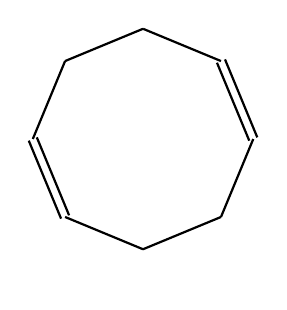
\begin{tikzpicture}[line width=.8pt,>=Stealth,baseline=(current bounding box.center)]
\draw (1.451,0.021)--(1.041,1.011);
\draw (1.349,-0.021)--(0.939,0.969);
\draw (0.990,0.990)--(0.000,1.400);
\draw (0.000,1.400)--(-0.990,0.990);
\draw (-0.990,0.990)--(-1.400,0.000);
\draw (-1.451,-0.021)--(-1.041,-1.011);
\draw (-1.349,0.021)--(-0.939,-0.969);
\draw (-0.990,-0.990)--(-0.000,-1.400);
\draw (-0.000,-1.400)--(0.990,-0.990);
\draw (0.990,-0.990)--(1.400,-0.000);
\node at(0.0,-1.7){$\mathrm{}$};
\end{tikzpicture}}\end{center}
\subsection*{独立推导}
\par 不饱和度为3；吸收2 mol氢对应两条可加氢双键，余下一重对应一个环。
\par 还原臭氧裂解将C=C两端变为羰基。唯一种类四碳二醛要求两段环链等长；把两分子丁二醛的两对醛端复接为双键，即得八元环两相对双键。
\subsection*{第三轮化学反校}
\par 一分子八碳底物实际给两分子四碳二醛；原“一个二醛”按一种产物理解，不误写只1 mol。
\par 加2H2后为环辛烷C8H16，碳氢和不饱和度均正确。
\subsection*{参考采分点（编辑建议）}
\par 下列为编辑建议，非原书官方评分。
\par 4分：DBE1；双键/环数1；二醛复接1；结构1。
\par\vspace{3mm}\footnotesize 来源：S01；PDF 156；印刷 150；题号8-64。\normalsize
\par\medskip\clearpage\subsection*{2．（10分）}将苯与氯甲烷在$\mathrm{AlCl_3}$作用下反应，分离后得到一个结晶，分子式为$\mathrm{C_{10}H_{14}}$；氢谱数据2.27(s,12H)、7.15(s,2H) ppm。根据以上数据和实验事实确定其结构式。

\subsection*{答案与边界}
1,2,4,5-四甲基苯（均四甲苯）。
\begin{center}\resizebox{.50\linewidth}{!}{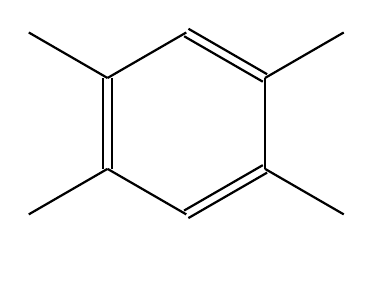
\begin{tikzpicture}[line width=.8pt,>=Stealth,baseline=(current bounding box.center)]
\draw (-2.000,-1.155)--(-1.000,-0.577);
\draw (-1.000,-0.577)--(-0.000,-1.155);
\draw (0.027,-1.202)--(1.027,-0.625);
\draw (-0.028,-1.107)--(0.972,-0.530);
\draw (1.000,-0.577)--(2.000,-1.155);
\draw (1.000,-0.577)--(1.000,0.577);
\draw (1.000,0.577)--(2.000,1.155);
\draw (1.027,0.625)--(0.028,1.202);
\draw (0.972,0.530)--(-0.027,1.107);
\draw (0.000,1.155)--(-1.000,0.577);
\draw (-1.000,0.577)--(-2.000,1.155);
\draw (-1.055,0.577)--(-1.055,-0.577);
\draw (-0.945,0.577)--(-0.945,-0.577);
\node at(0.0,-1.7){$\mathrm{}$};
\end{tikzpicture}}\end{center}
\subsection*{独立推导}
\par DBE=4。2.27的12H单峰对应4个芳甲基；另2H在芳香区，故苯环四取代。
\par 比较三种四甲基苯：1,2,4,5形式的对称操作可交换全部四Me及两芳H；另两种位置形式会分出不等价Me组。
\par 傅-克甲基化可继续多取代，分离产物事实与4Me相合；不能先假定只生成甲苯。
\subsection*{第三轮化学反校}
\par 6环C+4Me=10C，12甲基H+2芳H=14H。
\par 结晶本身不充分，判定主要依积分及对称性；未虚构熔点。
\subsection*{参考采分点（编辑建议）}
\par 下列为编辑建议，非原书官方评分。
\par 10分：DBE2；4Me积分2；取代对称性3；结构2；归属1。
\par\vspace{3mm}\footnotesize 来源：S01；PDF 341；印刷 335；题号16-53。\normalsize
\par\medskip\clearpage\subsection*{3．（10分）}分子式为$\mathrm{C_6H_{10}}$的A，加氢首先生成B($\mathrm{C_6H_{12}}$)，继续加氢至饱和生成C($\mathrm{C_6H_{14}}$)。A经臭氧化和还原水解生成两种醛D($\mathrm{C_2H_4O}$)和E($\mathrm{C_2H_2O_2}$)；B被高锰酸钾氧化只生成一种羧酸F($\mathrm{C_3H_6O_2}$)。试写出A—F六个化合物的构造式。

\subsection*{答案与边界}
A己-2,4-二烯；B己-3-烯；C正己烷；D乙醛；E乙二醛；F丙酸。E/Z未由原题决定。
\begin{center}\resizebox{.50\linewidth}{!}{\begin{tikzpicture}[line width=.8pt,>=Stealth,baseline=(current bounding box.center)]
\draw (-2.000,-0.129)--(-1.181,0.290);
\draw (-1.211,0.244)--(-0.439,-0.256);
\draw (-1.151,0.336)--(-0.379,-0.163);
\draw (-0.409,-0.209)--(0.409,0.209);
\draw (0.379,0.163)--(1.151,-0.336);
\draw (0.439,0.256)--(1.211,-0.244);
\draw (1.181,-0.290)--(2.000,0.129);
\node at(0.0,-1.7){$\mathrm{A}$};
\draw (3.800,-0.129)--(4.619,0.290);
\draw (4.619,0.290)--(5.391,-0.209);
\draw (5.416,-0.258)--(6.234,0.160);
\draw (5.366,-0.160)--(6.184,0.258);
\draw (6.209,0.209)--(6.981,-0.290);
\draw (6.981,-0.290)--(7.800,0.129);
\node at(5.8,-1.7){$\mathrm{B}$};
\draw (-2.000,-3.929)--(-1.181,-3.510);
\draw (-1.181,-3.510)--(-0.409,-4.009);
\draw (-0.409,-4.009)--(0.409,-3.591);
\draw (0.409,-3.591)--(1.181,-4.090);
\draw (1.181,-4.090)--(2.000,-3.671);
\node at(0.0,-5.5){$\mathrm{C}$};
\draw (3.800,-4.377)--(5.800,-3.223);
\draw (5.772,-3.270)--(7.772,-4.425);
\draw (5.827,-3.175)--(7.827,-4.330);
\node[fill=white,inner sep=1.1pt]at(7.800,-4.377){$\mathrm{O}$};
\node at(5.8,-5.5){$\mathrm{D}$};
\draw (2.022,-7.687)--(0.627,-7.094);
\draw (1.978,-7.789)--(0.584,-7.195);
\draw (0.606,-7.145)--(-0.606,-8.055);
\draw (-0.584,-8.005)--(-1.978,-7.411);
\draw (-0.627,-8.106)--(-2.022,-7.513);
\node[fill=white,inner sep=1.1pt]at(2.000,-7.738){$\mathrm{O}$};
\node[fill=white,inner sep=1.1pt]at(-2.000,-7.462){$\mathrm{O}$};
\node at(0.0,-9.299999999999999){$\mathrm{E}$};
\draw (3.800,-7.215)--(5.133,-6.445);
\draw (5.133,-6.445)--(6.467,-7.215);
\draw (6.412,-7.215)--(6.412,-8.755);
\draw (6.522,-7.215)--(6.522,-8.755);
\draw (6.467,-7.215)--(7.800,-6.445);
\node[fill=white,inner sep=1.1pt]at(6.467,-8.755){$\mathrm{O}$};
\node[fill=white,inner sep=1.1pt]at(7.800,-6.445){$\mathrm{OH}$};
\node at(5.8,-9.299999999999999){$\mathrm{F}$};
\end{tikzpicture}}\end{center}
\subsection*{独立推导}
\par B只有一个双键，强氧化给一种3C羧酸，须由对称六碳内烯断成两个丙酸，故B=己-3-烯，C=正己烷。
\par A比B少2H，另有一双键。乙二醛表示两双键之间为共轭CH=CH-CH=CH；两端乙醛使其成为CH3CH=CHCH=CHCH3。
\par 按题设观察A先生成B相当于共轭二烯1,4加氢。不能推广成所有催化剂下都只1,4加氢。
\subsection*{第三轮化学反校}
\par A臭氧给2乙醛+1乙二醛：4+2=6C，8+2=10H；原两种醛不是总两分子。
\par B的两个烯碳各有H，强氧化各得羧酸，产2丙酸；不混作还原臭氧醛。
\subsection*{参考采分点（编辑建议）}
\par 下列为编辑建议，非原书官方评分。
\par 10分：A2、B2、C1、D1、E1、F1；两裂解计量回代2。
\par\vspace{3mm}\footnotesize 来源：S03；PDF 170；印刷 165；题号2。\normalsize
\par\medskip\clearpage\subsection*{4．（5分）}下面是芳香化合物B($\mathrm{C_8H_8O_2}$)的$^1\mathrm H$ NMR图谱，指出化合物结构及图中各峰归属，并写出系统名称。
\begin{center}\resizebox{.87\linewidth}{!}{\begin{tikzpicture}[line width=.8pt,>=Stealth,baseline=(current bounding box.center)]
\draw(0,0)--(12,0);
\draw(12.0,0)--(12.0,-.12)node[below]{$0$};
\draw(10.8,0)--(10.8,-.12)node[below]{$1$};
\draw(9.6,0)--(9.6,-.12)node[below]{$2$};
\draw(8.4,0)--(8.4,-.12)node[below]{$3$};
\draw(7.2,0)--(7.2,-.12)node[below]{$4$};
\draw(6.0,0)--(6.0,-.12)node[below]{$5$};
\draw(4.8,0)--(4.8,-.12)node[below]{$6$};
\draw(3.6,0)--(3.6,-.12)node[below]{$7$};
\draw(2.4,0)--(2.4,-.12)node[below]{$8$};
\draw(1.2,0)--(1.2,-.12)node[below]{$9$};
\draw(0.0,0)--(0.0,-.12)node[below]{$10$};
\node at(6,-1.5){$\delta$};
\draw[blue!60!black,line width=.5pt](0.14399999999999907,0)--(0.14399999999999907,1.5);
\node[above,align=center,font=\scriptsize,rotate=90,anchor=west]at(0.14399999999999907,1.65){$9.880$};
\draw[red!50!black](-0.10600000000000093,0.2)--(0.08399999999999908,0.2)--(0.19399999999999906,0.30000000000000004)--(0.44399999999999906,0.30000000000000004);
\node[below,font=\scriptsize]at(0.14399999999999907,-.8){1.003};
\draw[blue!60!black,line width=.5pt](2.6111999999999993,0)--(2.6111999999999993,1.1);
\draw[blue!60!black,line width=.5pt](2.586,0)--(2.586,1.1);
\node[above,align=center,font=\scriptsize,rotate=90,anchor=west]at(2.5986,1.25){$7.845,7.824$};
\draw[red!50!black](2.3486,0.30000000000000004)--(2.5385999999999997,0.30000000000000004)--(2.6485999999999996,0.5)--(2.8985999999999996,0.5);
\node[below,font=\scriptsize]at(2.5986,-.8){2.000};
\draw[blue!60!black,line width=.5pt](3.6119999999999997,0)--(3.6119999999999997,1.1);
\draw[blue!60!black,line width=.5pt](3.5855999999999995,0)--(3.5855999999999995,1.1);
\node[above,align=center,font=\scriptsize,rotate=90,anchor=west]at(3.5987999999999998,1.25){$7.012,6.990$};
\draw[red!50!black](3.3487999999999998,0.5)--(3.5387999999999997,0.5)--(3.6487999999999996,0.7)--(3.8987999999999996,0.7);
\node[below,font=\scriptsize]at(3.5987999999999998,-.8){2.008};
\draw[blue!60!black,line width=.5pt](7.3427999999999995,0)--(7.3427999999999995,2.8);
\node[above,align=center,font=\scriptsize,rotate=90,anchor=west]at(7.3427999999999995,2.9499999999999997){$3.881$};
\draw[red!50!black](7.0927999999999995,0.7)--(7.2828,0.7)--(7.392799999999999,1.0)--(7.642799999999999,1.0);
\node[below,font=\scriptsize]at(7.3427999999999995,-.8){3.000};
\draw[blue!60!black,line width=.45pt](11.92,0)--(11.95,0)--(11.97,0.16)--(11.99,0)--(12.02,0);\draw[blue!60!black,line width=.45pt](9.42,0)--(9.45,.09)--(9.48,0);
\end{tikzpicture}}\end{center}
\subsection*{答案与边界}
B为4-甲氧基苯甲醛。
\begin{center}\resizebox{.50\linewidth}{!}{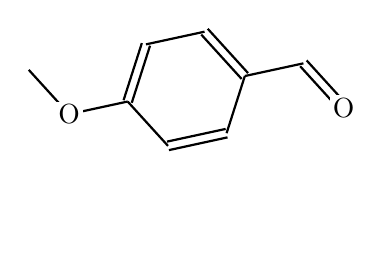
\begin{tikzpicture}[line width=.8pt,>=Stealth,baseline=(current bounding box.center)]
\draw (-2.000,0.240)--(-1.488,-0.323);
\draw (-1.488,-0.323)--(-0.744,-0.162);
\draw (-0.744,-0.162)--(-0.232,-0.725);
\draw (-0.220,-0.779)--(0.524,-0.617);
\draw (-0.244,-0.671)--(0.500,-0.510);
\draw (0.512,-0.564)--(0.744,0.162);
\draw (0.744,0.162)--(1.488,0.323);
\draw (1.447,0.286)--(1.959,-0.277);
\draw (1.529,0.360)--(2.041,-0.203);
\draw (0.785,0.199)--(0.273,0.762);
\draw (0.703,0.125)--(0.191,0.688);
\draw (0.232,0.725)--(-0.512,0.564);
\draw (-0.564,0.580)--(-0.796,-0.145);
\draw (-0.460,0.547)--(-0.692,-0.178);
\node[fill=white,inner sep=1.1pt]at(-1.488,-0.323){$\mathrm{O}$};
\node[fill=white,inner sep=1.1pt]at(2.000,-0.240){$\mathrm{O}$};
\node at(0.0,-1.7){$\mathrm{}$};
\end{tikzpicture}}\end{center}
\subsection*{独立推导}
\par DBE=5，可由苯环4+羰基1组成。9.880单峰积分约1为醛H，3.881单峰积分约3为OMe。
\par 芳区两个各2H双峰限定对位二取代苯环，苯6C+醛1C+OMe1C=8C。
\par H-2/6邻CHO：7.845/7.824；H-3/5邻OMe：7.012/6.990；CHO为9.880；OMe为3.881。
\subsection*{第三轮化学反校}
\par 积分1.003+2.000+2.008+3.000约8H，保留原实测尾差。
\par 谱图逐个保留原标ppm及积分，未以常见教科书整数位移替换原数据。
\subsection*{参考采分点（编辑建议）}
\par 下列为编辑建议，非原书官方评分。
\par 5分：DBE1；CHO/OMe1；对位判断1；结构名称1；逐峰归属1。
\par\vspace{3mm}\footnotesize 来源：S01；PDF 74,75；印刷 68,69；题号5-51。\normalsize
\par\medskip\clearpage\subsection*{5．（6分）}A($\mathrm{C_5H_8O_2}$)既能发生碘仿，又能发生银镜反应；经硼氢化钠还原成B($\mathrm{C_5H_{12}O_2}$)，B与浓硫酸生成C($\mathrm{C_5H_8}$)。C使溴水褪色但不与硝酸银氨溶液作用；强氧化除一分子$\mathrm{CO_2}$及$\mathrm{H_2O}$外，还得乙酸和乙二酸。推导A、B、C结构及有关反应式。

\subsection*{答案与边界}
A=4-氧代戊醛；B=戊烷-1,4-二醇；C=戊-1,3-二烯（E/Z未定）。
\begin{center}\resizebox{.50\linewidth}{!}{\begin{tikzpicture}[line width=.8pt,>=Stealth,baseline=(current bounding box.center)]
\draw (2.000,0.721)--(1.221,0.209);
\draw (1.166,0.206)--(1.220,-0.724);
\draw (1.276,0.212)--(1.330,-0.717);
\draw (1.221,0.209)--(0.389,0.628);
\draw (0.389,0.628)--(-0.389,0.117);
\draw (-0.389,0.117)--(-1.221,0.535);
\draw (-1.252,0.581)--(-2.030,0.070);
\draw (-1.191,0.489)--(-1.970,-0.022);
\node[fill=white,inner sep=1.1pt]at(1.275,-0.721){$\mathrm{O}$};
\node[fill=white,inner sep=1.1pt]at(-2.000,0.024){$\mathrm{O}$};
\node at(0.0,-1.7){$\mathrm{A}$};
\draw (7.800,0.721)--(7.021,0.209);
\draw (7.021,0.209)--(7.075,-0.721);
\draw (7.021,0.209)--(6.189,0.628);
\draw (6.189,0.628)--(5.411,0.117);
\draw (5.411,0.117)--(4.579,0.535);
\draw (4.579,0.535)--(3.800,0.024);
\node[fill=white,inner sep=1.1pt]at(7.075,-0.721){$\mathrm{OH}$};
\node[fill=white,inner sep=1.1pt]at(3.800,0.024){$\mathrm{OH}$};
\node at(5.8,-1.7){$\mathrm{B}$};
\draw (-1.972,-4.136)--(-0.973,-3.559);
\draw (-2.027,-4.041)--(-1.028,-3.464);
\draw (-1.000,-3.511)--(0.000,-4.089);
\draw (0.028,-4.136)--(1.028,-3.559);
\draw (-0.028,-4.041)--(0.973,-3.464);
\draw (1.000,-3.511)--(2.000,-4.089);
\node at(0.0,-5.5){$\mathrm{C}$};
\end{tikzpicture}}\end{center}
\subsection*{独立推导}
\par DBE(A)=2。银镜指向CHO，碘仿指向CH3CO；NaBH4使分子增加4H而保留2O，符合两个羰基分别还原成醇。
\par C由二醇脱2H2O形成两重不饱和；银炔阴性不单独排除所有内炔，需联用氧化片段。末端碳成CO2，中间两H碳成乙二酸，另一端成乙酸，反拼C为CH2=CHCH=CHCH3。
\par 在C1/C4逆加羟基得二醇B，再将伯醇氧化为CHO、仲醇氧化为甲基酮得A。
\subsection*{第三轮化学反校}
\par C裂解碳数1+2+2=5；B−2H2O=C5H8，A+4H=B。
\par 只按题设给出能解释观察的反应链，不虚称酸脱水无副反应或有测定选择性收率。
\subsection*{参考采分点（编辑建议）}
\par 下列为编辑建议，非原书官方评分。
\par 6分：A2；B1；C及裂解2；守恒1。
\par\vspace{3mm}\footnotesize 来源：S03；PDF 109；印刷 104；题号4。\normalsize
\par\medskip\clearpage\clearpage\section*{四、简答与分析（3题，共15分）}\subsection*{1．（5分）}北大习题3-5\quad 印刷28页/PDF34页。\par\bigskip
画出以新戊烷分子中某根$\mathrm{C-C}$键为轴旋转$360^\circ$时各种构象的势能关系图。

\par\bigskip\textbf{答案：}每$120^\circ$重复；三等价重叠为峰，三等价交错为谷。
\begin{center}\begin{tikzpicture}[line width=.8pt,>=Stealth]\draw[->](0,0)--(10.2,0)node[right]{角度};\draw[->](0,0)--(0,2.6)node[above]{相对势能};\draw[thick,domain=0:360,samples=121]plot({\x/36},{1.1*(1+cos(3*\x))});\foreach \a in{0,60,120,180,240,300,360}{\draw({\a/36},0)--({\a/36},-.1)node[below]{$\a^\circ$};}\node[left]at(0,0){$0$};\node[left]at(0,2.2){$E_{\rm b}$};\end{tikzpicture}\end{center}\begin{center}\begin{tikzpicture}[line width=.8pt,>=Stealth]\draw(0.0,0)circle(.33);
\fill(0.0,0)circle(.03);
\draw(0.0,0.0)--(4.7761225166746774e-17,0.78);
\node[fill=white,inner sep=1pt]at(6.000769315822031e-17,0.98){$\mathrm{H/Me}$};
\draw(0.0,0.0)--(-0.6754998149518622,-0.3900000000000001);
\node[fill=white,inner sep=1pt]at(-0.8487048957087499,-0.4900000000000001){$\mathrm{H/Me}$};
\draw(0.0,0.0)--(0.675499814951862,-0.39000000000000035);
\node[fill=white,inner sep=1pt]at(0.8487048957087496,-0.49000000000000044){$\mathrm{H/Me}$};
\draw(2.020667218593133e-17,0.33)--(4.7761225166746774e-17,0.78);
\draw(-0.28578838324886474,-0.16500000000000004)--(-0.6754998149518622,-0.3900000000000001);
\draw(0.2857883832488647,-0.16500000000000015)--(0.675499814951862,-0.39000000000000035);
\node at(0.0,-1.35){$0^\circ$重叠};
\draw(3.3,0)circle(.33);
\fill(3.3,0)circle(.03);
\draw(3.3,0.0)--(3.3,0.78);
\node[fill=white,inner sep=1pt]at(3.3,0.98){$\mathrm{H}$};
\draw(3.3,0.0)--(2.6245001850481375,-0.3900000000000001);
\node[fill=white,inner sep=1pt]at(2.45129510429125,-0.4900000000000001){$\mathrm{H}$};
\draw(3.3,0.0)--(3.9754998149518617,-0.39000000000000035);
\node[fill=white,inner sep=1pt]at(4.148704895708749,-0.49000000000000044){$\mathrm{H}$};
\draw(3.014211616751135,0.16499999999999998)--(2.6245001850481375,0.38999999999999996);
\node[fill=white,inner sep=1pt]at(2.45129510429125,0.48999999999999994){$\mathrm{Me}$};
\draw(3.3,-0.33)--(3.3,-0.78);
\node[fill=white,inner sep=1pt]at(3.3,-0.98){$\mathrm{Me}$};
\draw(3.5857883832488646,0.165)--(3.975499814951862,0.39);
\node[fill=white,inner sep=1pt]at(4.148704895708749,0.49){$\mathrm{Me}$};
\node at(3.3,-1.35){$60^\circ$交错};
\draw(6.6,0)circle(.33);
\fill(6.6,0)circle(.03);
\draw(6.6,0.0)--(6.6,0.78);
\node[fill=white,inner sep=1pt]at(6.6,0.98){$\mathrm{H/Me}$};
\draw(6.6,0.0)--(5.924500185048138,-0.3900000000000001);
\node[fill=white,inner sep=1pt]at(5.75129510429125,-0.4900000000000001){$\mathrm{H/Me}$};
\draw(6.6,0.0)--(7.2754998149518615,-0.39000000000000035);
\node[fill=white,inner sep=1pt]at(7.448704895708749,-0.49000000000000044){$\mathrm{H/Me}$};
\draw(6.314211616751135,-0.16500000000000004)--(5.924500185048138,-0.3900000000000001);
\draw(6.885788383248864,-0.16500000000000015)--(7.2754998149518615,-0.39000000000000035);
\draw(6.6,0.33)--(6.6,0.78);
\node at(6.6,-1.35){$120^\circ$重叠};
\draw(0.0,-3)circle(.33);
\fill(0.0,-3)circle(.03);
\draw(0.0,-3.0)--(4.7761225166746774e-17,-2.2199999999999998);
\node[fill=white,inner sep=1pt]at(6.000769315822031e-17,-2.02){$\mathrm{H}$};
\draw(0.0,-3.0)--(-0.6754998149518622,-3.39);
\node[fill=white,inner sep=1pt]at(-0.8487048957087499,-3.49){$\mathrm{H}$};
\draw(0.0,-3.0)--(0.675499814951862,-3.3900000000000006);
\node[fill=white,inner sep=1pt]at(0.8487048957087496,-3.49){$\mathrm{H}$};
\draw(-6.062001655779399e-17,-3.33)--(-1.4328367550024033e-16,-3.7800000000000002);
\node[fill=white,inner sep=1pt]at(-1.8002307947466092e-16,-3.98){$\mathrm{Me}$};
\draw(0.28578838324886474,-2.835)--(0.6754998149518622,-2.61);
\node[fill=white,inner sep=1pt]at(0.8487048957087499,-2.51){$\mathrm{Me}$};
\draw(-0.2857883832488648,-2.835)--(-0.6754998149518623,-2.6100000000000003);
\node[fill=white,inner sep=1pt]at(-0.8487048957087501,-2.5100000000000002){$\mathrm{Me}$};
\node at(0.0,-4.35){$180^\circ$交错};
\draw(3.3,-3)circle(.33);
\fill(3.3,-3)circle(.03);
\draw(3.3,-3.0)--(3.3,-2.2199999999999998);
\node[fill=white,inner sep=1pt]at(3.3,-2.02){$\mathrm{H/Me}$};
\draw(3.3,-3.0)--(2.6245001850481375,-3.39);
\node[fill=white,inner sep=1pt]at(2.45129510429125,-3.49){$\mathrm{H/Me}$};
\draw(3.3,-3.0)--(3.9754998149518617,-3.3900000000000006);
\node[fill=white,inner sep=1pt]at(4.148704895708749,-3.49){$\mathrm{H/Me}$};
\draw(3.5857883832488646,-3.165)--(3.9754998149518617,-3.3900000000000006);
\draw(3.3,-2.67)--(3.3000000000000003,-2.2199999999999998);
\draw(3.014211616751135,-3.1649999999999996)--(2.624500185048137,-3.3899999999999992);
\node at(3.3,-4.35){$240^\circ$重叠};
\draw(6.6,-3)circle(.33);
\fill(6.6,-3)circle(.03);
\draw(6.6,-3.0)--(6.6,-2.2199999999999998);
\node[fill=white,inner sep=1pt]at(6.6,-2.02){$\mathrm{H}$};
\draw(6.6,-3.0)--(5.924500185048138,-3.39);
\node[fill=white,inner sep=1pt]at(5.75129510429125,-3.49){$\mathrm{H}$};
\draw(6.6,-3.0)--(7.2754998149518615,-3.3900000000000006);
\node[fill=white,inner sep=1pt]at(7.448704895708749,-3.49){$\mathrm{H}$};
\draw(6.885788383248864,-2.835)--(7.2754998149518615,-2.61);
\node[fill=white,inner sep=1pt]at(7.448704895708749,-2.51){$\mathrm{Me}$};
\draw(6.314211616751135,-2.835)--(5.924500185048137,-2.6100000000000003);
\node[fill=white,inner sep=1pt]at(5.751295104291249,-2.5100000000000002){$\mathrm{Me}$};
\draw(6.6,-3.33)--(6.6,-3.7800000000000002);
\node[fill=white,inner sep=1pt]at(6.6,-3.98){$\mathrm{Me}$};
\node at(6.6,-4.35){$300^\circ$交错};\end{tikzpicture}\end{center}\par 重叠型末端$\mathrm{H/Me}$表示前碳H与后碳Me沿视线重合。
\par\bigskip\textbf{从基础到判断：}\begin{enumerate}\item 从甲基碳向季碳观察：前碳三个H、后碳三个Me。轴键朝向视线，不额外画第四条径向键。
\item 旋转只改二面角不断键。重叠投影三对C–H/C–C重合，扭转及空间作用较大；交错错开$60^\circ$较有利。
\item 三个H及三个Me各自等价，故周期$120^\circ$。图取谷为零、峰为$E_{\rm b}$；原题未给实验值，不把书图15.9当普适实测。\end{enumerate}
\textbf{反向校核：}\begin{itemize}\item 轴两端各三条非轴键；0与360为同一构象；三峰等高、三谷等高。\end{itemize}
\textbf{参考采分点：}观察方向1分；六构象2分；峰谷周期2分。\par\medskip\clearpage\subsection*{2．（5分）}北大习题5-30\quad 印刷62页/PDF68页。\par\bigskip
游离羧酸$\mathrm{C=O}$的吸收频率为$1760\,\mathrm{cm^{-1}}$左右，而羧酸二聚体的$\mathrm{C=O}$吸收频率为$1700\,\mathrm{cm^{-1}}$左右，试阐明原因。

\par\bigskip\textbf{答案：}二聚氢键降低羰基有效力常数，使伸缩振动波数降低。
\begin{center}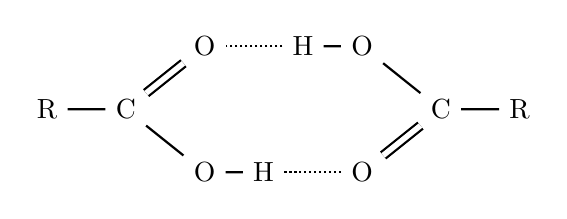
\begin{tikzpicture}[line width=.8pt,>=Stealth]\node(c1)at(-2,0){$\mathrm C$};\node(c2)at(2,0){$\mathrm C$};\node(o1)at(-1,.8){$\mathrm O$};\node(o2)at(-1,-.8){$\mathrm O$};\node(o3)at(1,-.8){$\mathrm O$};\node(o4)at(1,.8){$\mathrm O$};\node(h1)at(-.25,-.8){$\mathrm H$};\node(h2)at(.25,.8){$\mathrm H$};\node(r1)at(-3,0){$\mathrm R$};\node(r2)at(3,0){$\mathrm R$};\draw(r1)--(c1)--(o2)--(h1);\draw(r2)--(c2)--(o4)--(h2);\draw[densely dotted,thick](h1)--(o3);\draw[densely dotted,thick](h2)--(o1);\draw[double,double distance=2pt](c1)--(o1);\draw[double,double distance=2pt](c2)--(o3);\end{tikzpicture}\end{center}
\par\bigskip\textbf{从基础到判断：}\begin{enumerate}\item 羧酸兼有供体O–H和受体羰基O，两分子以两条O–H$\cdots$O氢键形成环状二聚体。虚点为分子间氢键而非共价键。
\item 羰基O接受氢键改变电子分布，C=O有效双键性及伸缩力常数降低。近似振子$\widetilde\nu=(2\pi c)^{-1}\sqrt{k/\mu}$；原子质量相同时，$k$降低使波数降低。
\item 1760及1700是题给近似值，不补造相态、溶剂和温度；红移不表示C=O完全断裂。\end{enumerate}
\textbf{反向校核：}\begin{itemize}\item 两C=O均保留；双互补氢键；不能将羰基约化质量因二聚直接加倍。\end{itemize}
\textbf{参考采分点：}二聚结构2分；电子/力常数2分；波数关系1分。\par\medskip\clearpage\subsection*{3．（5分）}北大习题6-13\quad 印刷85页/PDF91页。\par\bigskip
根据下表中数据判断四个溴代烷的水解反应各为几级反应。
\begin{center}\small 体积分数$80\%$乙醇的水溶液，$55\,{}^\circ\mathrm C$\par\medskip\begin{tabular}{lcc}\hline 溴代烷&$k_1/(10^{-5}\,\mathrm{s^{-1}})$&$k_2/(10^{-5}\,\mathrm{L\,mol^{-1}s^{-1}})$\\\hline $\mathrm{CH_3Br}$&0.35&2140\\$\mathrm{CH_3CH_2Br}$&0.14&171\\$\mathrm{(CH_3)_2CHBr}$&0.24&4.75\\$\mathrm{(CH_3)_3CBr}$&1010&（原表空白）\\\hline\end{tabular}\end{center}
\par\bigskip\textbf{答案：}教材主路线判断：叔丁基溴为一级；溴甲烷、溴乙烷、2-溴丙烷为二级。

\par\bigskip\textbf{从基础到判断：}\begin{enumerate}\item 一级模型$v=k_1[\mathrm{RBr}]$，$k_1$为$\mathrm{s^{-1}}$；二级模型$v=k_2[\mathrm{RBr}][\mathrm{Nu}]$，$k_2$为$\mathrm{L\,mol^{-1}s^{-1}}$。
\item 二级列从甲基2140经一级171降到二级4.75，符合背攻受位阻抑制的$\mathrm{S_N2}$趋势。叔丁基背攻拥挤，而一级列跃至1010，符合三级碳正离子较易形成的$\mathrm{S_N1}$溶剂解。
\item 两列量纲不同，不能直接比数字。单表不是浓度–速率原始测量，严格证明级数仍需改变浓度测速率；大量水恒定时二级过程也可能显示拟一级。\end{enumerate}
\textbf{反向校核：}\begin{itemize}\item 两列倍率均$10^{-5}$，两人独立放大核过；$80\%$是体积分数；55度；空白不补0；四底物全对应。\end{itemize}
\textbf{参考采分点：}四底物归类2分；结构趋势2分；速率式量纲1分。\par\medskip\clearpage\clearpage\section*{五、反应机理（3题，共18分）}\subsection*{1．（6分）}原书6-11，印刷[84]页；PDF[90]页。\par\medskip 画出由$(CH_3)_3CCH_2CH_2^+$转变为$(CH_3)_2C^+CH(CH_3)_2$的反应机理。\par\smallskip\begin{center}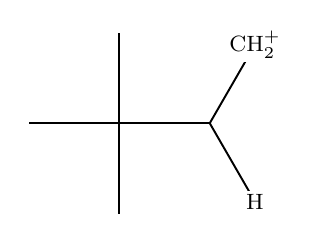
\begin{tikzpicture}[line width=.7pt,font=\footnotesize]\draw(-0.28750000000000014,8.511709855459533e-17)--(-0.2874999999999997,1.15);
\draw(-0.28750000000000014,8.511709855459533e-17)--(-0.2875000000000004,-1.15);
\draw(-0.28750000000000014,8.511709855459533e-17)--(-1.4375000000000002,2.55351295663786e-16);
\draw(-0.28750000000000014,8.511709855459533e-17)--(0.8624999999999999,-1.27675647831893e-16);
\draw(0.8624999999999999,-1.27675647831893e-16)--(1.4374999999999996,-0.9959292143521049);
\draw(0.8624999999999999,-1.27675647831893e-16)--(1.4375000000000002,0.9959292143521044);
\node[fill=white,inner sep=1.2pt]at(1.4374999999999996,-0.9959292143521049){$\mathrm{H}$};
\node[fill=white,inner sep=1.2pt]at(1.4375000000000002,0.9959292143521044){$\mathrm{CH_{2}^{+}}$};\end{tikzpicture}\end{center}\par\smallskip \par\medskip\begin{samepage}\subsection*{步骤1　1,2-氢负迁移}
\begin{center}\resizebox{.96\linewidth}{!}{\begin{tikzpicture}[line width=.7pt,font=\footnotesize]
\draw(-0.28750000000000014,8.511709855459533e-17)--(-0.2874999999999997,1.15);
\draw(-0.28750000000000014,8.511709855459533e-17)--(-0.2875000000000004,-1.15);
\draw(-0.28750000000000014,8.511709855459533e-17)--(-1.4375000000000002,2.55351295663786e-16);
\draw(-0.28750000000000014,8.511709855459533e-17)--(0.8624999999999999,-1.27675647831893e-16);
\draw(0.8624999999999999,-1.27675647831893e-16)--(1.4374999999999996,-0.9959292143521049);
\draw(0.8624999999999999,-1.27675647831893e-16)--(1.4375000000000002,0.9959292143521044);
\node[fill=white,inner sep=1.2pt]at(1.4374999999999996,-0.9959292143521049){$\mathrm{H}$};
\node[fill=white,inner sep=1.2pt]at(1.4375000000000002,0.9959292143521044){$\mathrm{CH_{2}^{+}}$};
\draw(6.9368252301841835,6.882655855347339e-17)--(6.473386700693274,1.15);
\draw(6.9368252301841835,6.882655855347339e-17)--(7.400263759675094,-1.15);
\draw(6.9368252301841835,6.882655855347339e-17)--(5.786825230184184,-0.46343852949090986);
\draw(6.9368252301841835,6.882655855347339e-17)--(8.086825230184184,0.4634385294909099);
\draw(8.086825230184184,0.4634385294909099)--(9.063174769815816,-0.30077142011573993);
\draw(9.063174769815816,-0.30077142011573993)--(10.213174769815815,0.16266710937516998);
\node[fill=white,inner sep=1.2pt]at(8.086825230184184,0.4634385294909099){$\mathrm{CH^{+}}$};
\node[fill=white,inner sep=1.2pt]at(10.213174769815815,0.16266710937516998){$\mathrm{H}$};
\draw[->,thick](3.2,0)--(4.6,0);
\draw[-{Stealth[length=1.7mm]},blue!70!black](1.1499999999999997,-0.4979646071760525)to[bend left=40](1.4375000000000002,1.1659292143521043);
\end{tikzpicture}}\end{center}相邻C—H键的一对电子带着H迁至末端缺电子碳。原一级正电中心变饱和，正电荷留在原给氢的碳，得到二级碳正离子。不是H+游离后再加成。\par\medskip\end{samepage}
\begin{samepage}\subsection*{步骤2　1,2-甲基迁移}
\begin{center}\resizebox{.96\linewidth}{!}{\begin{tikzpicture}[line width=.7pt,font=\footnotesize]
\draw(-1.063174769815816,6.882655855347339e-17)--(-1.5266132993067258,1.15);
\draw(-1.063174769815816,6.882655855347339e-17)--(-0.599736240324906,-1.15);
\draw(-1.063174769815816,6.882655855347339e-17)--(-2.213174769815816,-0.46343852949090986);
\draw(-1.063174769815816,6.882655855347339e-17)--(0.08682523018418424,0.4634385294909099);
\draw(0.08682523018418424,0.4634385294909099)--(1.063174769815816,-0.30077142011573993);
\draw(1.063174769815816,-0.30077142011573993)--(2.213174769815816,0.16266710937516998);
\node[fill=white,inner sep=1.2pt]at(0.08682523018418424,0.4634385294909099){$\mathrm{CH^{+}}$};
\node[fill=white,inner sep=1.2pt]at(2.213174769815816,0.16266710937516998){$\mathrm{H}$};
\draw(7.024259474352178,0.15249195864350237)--(6.800513031644505,1.15);
\draw(7.024259474352178,0.15249195864350237)--(6.272265391412029,-0.5400321654259905);
\draw(7.024259474352178,0.15249195864350237)--(8.0,-0.15249195864350226);
\draw(8.0,-0.15249195864350226)--(8.223746442707673,-1.15);
\draw(8.0,-0.15249195864350226)--(8.751994082940149,0.5400321654259914);
\draw(8.751994082940149,0.5400321654259914)--(9.727734608587971,0.2350482481389867);
\node[fill=white,inner sep=1.2pt]at(7.024259474352178,0.15249195864350237){$\mathrm{C^{+}}$};
\node[fill=white,inner sep=1.2pt]at(9.727734608587971,0.2350482481389867){$\mathrm{H}$};
\draw[->,thick](3.2,0)--(4.6,0);
\draw[-{Stealth[length=1.7mm]},blue!70!black](-1.294894034561271,0.575)to[bend left=-40](0.08682523018418424,0.63343852949091);
\end{tikzpicture}}\end{center}邻位季碳的一根C—Me键带电子迁向二级正离子中心；原季碳失去这根键而成为三级碳正离子，碳骨架重新连接。\par\medskip\end{samepage}
\textbf{化学反校：}两步均保留6C、总+1；先氢迁移再甲基迁移，不能一步凭空跨两碳迁移。每根弯箭从实际$\sigma$键出发，终点是相邻缺电子中心。\par\textbf{6分参考采分：}H迁移及中间体2分;Me迁移及产物2分;两步电子箭头/价态各1分\par\textbf{边界：}\par\medskip\clearpage\subsection*{2．（6分）}原书8-13，印刷[134]页；PDF[140]页。\par\medskip 苯乙烯在甲醇溶液中溴化，得到1-苯基-1,2-二溴乙烷及1-苯基-1-甲氧基-2-溴乙烷。写出反应机理。\par\smallskip\begin{center}\begin{tikzpicture}[line width=.7pt,font=\footnotesize]\draw(-2.2039332610057802,0.32463006733740674)--(-1.3870118242547032,-0.5604204984175614);
\draw(-2.1377991516046895,0.3856733271924029)--(-1.3208777148536124,-0.4993772385625652);
\draw(-1.3539447695541578,-0.5298988684900633)--(-0.17900777760102723,-0.2649494342450316);
\draw(-0.21207483230157254,-0.29547106417252966)--(0.604846604449505,-1.1805216299274979);
\draw(-0.14594072290048193,-0.23442780431753352)--(0.6709807138505955,-1.119478370072502);
\draw(0.6379136591500503,-1.15)--(1.8128506511031812,-0.8850505657549682);
\draw(1.8558166853355746,-0.898426660190221)--(2.213832240537628,0.2515733398097787);
\draw(1.7698846168707878,-0.8716744713197154)--(2.1279001720728417,0.2783255286802844);
\draw(2.170866206305235,0.26494943424503153)--(1.3539447695541578,1.15);
\draw(1.3440457900223097,1.1938977243627509)--(0.16910879806917892,0.9289482901177198);
\draw(1.3638437490860058,1.106102275637249)--(0.188906757132875,0.8411528413922181);
\draw(0.17900777760102696,0.885050565754969)--(-0.17900777760102723,-0.2649494342450316);\end{tikzpicture}\end{center}\par\smallskip \par\medskip\begin{samepage}\subsection*{步骤1　溴正离子桥形成}
\begin{center}\resizebox{.96\linewidth}{!}{\begin{tikzpicture}[line width=.7pt,font=\footnotesize]
\draw(-0.9705144061978873,-0.659842191803252)--(-1.5760392602167563,-0.00381813548828246);
\draw(-1.036648515598978,-0.7208854516582481)--(-1.642173369617847,-0.06486139534327859);
\draw(-1.0035814608984326,-0.6903638217307501)--(-0.1326855356265215,-0.4939759436850303);
\draw(-0.1657525903270668,-0.5244975736125284)--(0.43977226369180245,-1.1805216299274979);
\draw(-0.09961848092597621,-0.4634543137575322)--(0.505906373092893,-1.119478370072502);
\draw(0.4728393183923477,-1.15)--(1.3437352436642591,-0.9536121219542801);
\draw(1.3867012778966525,-0.966988216389533)--(1.6520723491496951,-0.11457628202884367);
\draw(1.3007692094318657,-0.9402360275190272)--(1.5661402806849083,-0.08782409315833799);
\draw(1.6091063149173017,-0.10120018759359083)--(1.0035814608984326,0.5548238687213788);
\draw(0.9936824813665845,0.5987215930841296)--(0.12278655609467325,0.4023337150384105);
\draw(1.0134804404302806,0.5109261443586279)--(0.14258451515836934,0.31453826631290865);
\draw(-0.21931027820188992,1.15)--(0.6734539187160417,1.15);
\draw(0.1326855356265213,0.35843599067565957)--(-0.1326855356265215,-0.4939759436850303);
\node[fill=white,inner sep=1.2pt]at(-0.21931027820188992,1.15){$\mathrm{Br}$};
\node[fill=white,inner sep=1.2pt]at(0.6734539187160417,1.15){$\mathrm{Br}$};
\draw(9.853460969082652,0.15980762113533195)--(9.023076211353315,-0.31961524227066274);
\draw(9.023076211353315,-0.31961524227066274)--(8.064230484541326,-0.31961524227066285);
\draw(8.103201627711627,-0.2971152422706629)--(7.623778764305632,0.5332695154586736);
\draw(8.025259341371026,-0.3421152422706628)--(7.545836477965032,0.4882695154586737);
\draw(7.584807621135332,0.5107695154586737)--(6.625961894323343,0.5107695154586738);
\draw(6.586990751153043,0.5332695154586737)--(6.107567887747048,-0.2971152422706627);
\draw(6.664933037493642,0.48826951545867375)--(6.185510174087647,-0.34211524227066276);
\draw(6.1465390309173475,-0.31961524227066274)--(6.625961894323342,-1.1499999999999992);
\draw(6.625961894323342,-1.1949999999999992)--(7.584807621135331,-1.1949999999999998);
\draw(6.625961894323342,-1.1049999999999993)--(7.584807621135331,-1.105);
\draw(9.023076211353315,-0.31961524227066274)--(9.853460969082652,-0.7990381056766573);
\draw(9.853460969082652,-0.7990381056766573)--(9.853460969082652,0.15980762113533195);
\draw(7.584807621135331,-1.15)--(8.064230484541326,-0.31961524227066285);
\node[fill=white,inner sep=1.2pt]at(9.853460969082652,0.15980762113533195){$\mathrm{Br^{+}}$};
\node[fill=white,inner sep=1.2pt]at(7.929145188432738,1.15){$\mathrm{Br^{-}}$};
\draw[->,thick](3.2,0)--(4.6,0);
\draw[-{Stealth[length=1.7mm]},blue!70!black](-1.3063438879078673,-0.3623517935732653)to[bend left=35](-0.21931027820188992,1.3199999999999998);
\draw[-{Stealth[length=1.7mm]},blue!70!black](0.22707182025707587,1.15)to[bend left=-25](0.6734539187160417,1.3199999999999998);
\draw[-{Stealth[length=1.7mm]},blue!70!black](-0.21931027820188992,1.3199999999999998)to[bend left=30](-1.6091063149173017,0.1356602345842195);
\node[blue!70!black]at(-0.3493102782018899,1.41){:};
\end{tikzpicture}}\end{center}双键$\pi$电子进攻被极化的Br，Br—Br异裂；所连Br用孤电子同时桥连另一烯碳，形成三元溴正离子离子。两面均可进攻，不能指定单一构型。\par\medskip\end{samepage}
\begin{samepage}\subsection*{步骤2　支路I：Br$-$背面开桥}
\begin{center}\resizebox{.96\linewidth}{!}{\begin{tikzpicture}[line width=.7pt,font=\footnotesize]
\draw(1.8534609690826525,0.15980762113533195)--(1.0230762113533154,-0.31961524227066274);
\draw(1.0230762113533154,-0.31961524227066274)--(0.06423048454132634,-0.31961524227066285);
\draw(0.10320162771162608,-0.2971152422706628)--(-0.37622123569436844,0.5332695154586736);
\draw(0.025259341371026596,-0.34211524227066287)--(-0.45416352203496796,0.48826951545867364);
\draw(-0.4151923788646682,0.5107695154586737)--(-1.3740381056766575,0.5107695154586738);
\draw(-1.4130092488469572,0.5332695154586737)--(-1.8924321122529522,-0.2971152422706627);
\draw(-1.3350669625063578,0.48826951545867375)--(-1.8144898259123527,-0.34211524227066276);
\draw(-1.8534609690826525,-0.31961524227066274)--(-1.374038105676658,-1.1499999999999992);
\draw(-1.374038105676658,-1.1949999999999992)--(-0.41519237886466903,-1.1949999999999998);
\draw(-1.374038105676658,-1.1049999999999993)--(-0.4151923788646689,-1.105);
\draw(1.0230762113533154,-0.31961524227066274)--(1.8534609690826518,-0.7990381056766573);
\draw(1.8534609690826518,-0.7990381056766573)--(1.8534609690826525,0.15980762113533195);
\draw(-0.415192378864669,-1.15)--(0.06423048454132634,-0.31961524227066285);
\node[fill=white,inner sep=1.2pt]at(1.8534609690826525,0.15980762113533195){$\mathrm{Br^{+}}$};
\node[fill=white,inner sep=1.2pt]at(-0.0708548115672621,1.15){$\mathrm{Br^{-}}$};
\draw(7.25421047812743,-0.14441821878806949)--(8.331976404784035,-1.307859708409841e-16);
\draw(8.296338732080962,-0.027476467828101363)--(8.960291541649031,-0.8886400302519628);
\draw(8.367614077487108,0.0274764678281011)--(9.031566887055178,-0.8336870945957604);
\draw(8.995929214352104,-0.8611635624238616)--(10.07369514100871,-0.7167453436357926);
\draw(10.115309296505647,-0.7338702396143579)--(10.529122413594182,0.27171154159757277);
\draw(10.032080985511772,-0.6996204476572272)--(10.445894102600308,0.3059613335547036);
\draw(10.487508258097245,0.2888364375761382)--(9.823555448529175,1.15);
\draw(9.81757896573531,1.1946013638066666)--(8.739813039078705,1.0501831450185979);
\draw(9.829531931323041,1.1053986361933332)--(8.751766004666436,0.9609804174052645);
\draw(7.25421047812743,-0.14441821878806949)--(6.840397361038894,-1.15);
\draw(7.25421047812743,-0.14441821878806949)--(6.59025766855936,0.7167453436357921);
\draw(6.59025766855936,0.7167453436357921)--(5.512491741902755,0.5723271248477226);
\draw(8.74578952187257,1.0055817812119312)--(8.331976404784035,-1.307859708409841e-16);
\node[fill=white,inner sep=1.2pt]at(6.840397361038894,-1.15){$\mathrm{Br}$};
\node[fill=white,inner sep=1.2pt]at(5.512491741902755,0.5723271248477226){$\mathrm{Br}$};
\draw[->,thick](3.2,0)--(4.6,0);
\draw[-{Stealth[length=1.7mm]},blue!70!black](-0.0708548115672621,1.3199999999999998)to[bend left=35](1.0230762113533154,-0.14961524227066272);
\node[blue!70!black]at(-0.2008548115672621,1.41){:};
\draw[-{Stealth[length=1.7mm]},blue!70!black](1.438268590217984,-0.07990381056766539)to[bend left=-35](1.8534609690826525,0.32980762113533196);
\end{tikzpicture}}\end{center}Br$-$从桥Br反面进攻较稳定的苄位碳，断开该碳—桥Br键，形成邻二溴物；苄位形成外消旋对。\par\medskip\end{samepage}
\begin{samepage}\subsection*{步骤3　支路II：甲醇背面开桥}
\begin{center}\resizebox{.96\linewidth}{!}{\begin{tikzpicture}[line width=.7pt,font=\footnotesize]
\draw(1.2469706036295638,-0.2687882414518254)--(0.6883047348235801,-0.591334131194016);
\draw(0.6883047348235801,-0.591334131194016)--(0.04321295533919896,-0.5913341311940161);
\draw(0.0821840985094987,-0.5688341311940162)--(-0.24036179123269188,-0.010168262388032808);
\draw(0.004241812168899219,-0.6138341311940161)--(-0.3183040775732914,-0.055168262388032796);
\draw(-0.2793329344029916,-0.032668262388032804)--(-0.9244247138873729,-0.03266826238803271);
\draw(-0.9633958570576726,-0.010168262388032697)--(-1.2859417467998635,-0.568834131194016);
\draw(-0.8854535707170732,-0.05516826238803271)--(-1.207999460459264,-0.613834131194016);
\draw(-1.2469706036295638,-0.591334131194016)--(-0.9244247138873734,-1.1499999999999995);
\draw(-0.9244247138873734,-1.1949999999999994)--(-0.27933293440299223,-1.1949999999999998);
\draw(-0.9244247138873734,-1.1049999999999995)--(-0.2793329344029921,-1.105);
\draw(0.6883047348235801,-0.591334131194016)--(1.2469706036295634,-0.9138800209362068);
\draw(-0.047669666976487494,0.7199388136770789)--(0.5109962018294959,0.397392923934888);
\draw(-0.047669666976487494,0.7199388136770789)--(-0.6063355357824708,0.3973929239348884);
\draw(1.2469706036295634,-0.9138800209362068)--(1.2469706036295638,-0.2687882414518254);
\draw(-0.2793329344029922,-1.15)--(0.04321295533919896,-0.5913341311940161);
\node[fill=white,inner sep=1.2pt]at(1.2469706036295638,-0.2687882414518254){$\mathrm{Br^{+}}$};
\node[fill=white,inner sep=1.2pt]at(-0.047669666976487494,1.15){$\mathrm{Br^{-}}$};
\node[fill=white,inner sep=1.2pt]at(-0.047669666976487494,0.7199388136770789){$\mathrm{O}$};
\node[fill=white,inner sep=1.2pt]at(0.5109962018294959,0.397392923934888){$\mathrm{H}$};
\draw(8.49401731143733,-0.49175091515536357)--(7.809979856835563,-0.4478474004757235);
\draw(7.850312127563292,-0.4278897468574961)--(7.546314959290399,0.18645582330749996);
\draw(7.769647586107833,-0.46780505409395096)--(7.46565041783494,0.1465405160710451);
\draw(7.5059826885626695,0.16649816968927253)--(6.821945233960902,0.21040168436891296);
\draw(6.784495263563722,0.23535162860232442)--(6.404454977234845,-0.33509042688303153);
\draw(6.859395204358082,0.1854517401355015)--(6.479354918029205,-0.38499031534985445);
\draw(6.441904947632025,-0.360040371116443)--(6.745902115904918,-0.9743859412814393);
\draw(6.743019815574368,-1.0192935391330782)--(7.427057270176137,-1.0631970538127185);
\draw(6.748784416235467,-0.9294783434298005)--(7.432821870837236,-0.9733818581094408);
\draw(8.49401731143733,-0.49175091515536357)--(8.874057597766207,0.07869114032999217);
\draw(8.874057597766207,0.07869114032999217)--(9.558095052367975,0.03478762565035178);
\draw(8.874057597766207,0.07869114032999217)--(8.570060429493314,0.6930367104949887);
\draw(8.49401731143733,-0.49175091515536357)--(8.798014479710224,-1.1060964853203596);
\draw(8.798014479710224,-1.1060964853203596)--(9.482051934311992,-1.15);
\draw(7.429939570506686,-1.0182894559610796)--(7.809979856835563,-0.4478474004757235);
\node[fill=white,inner sep=1.2pt]at(8.874057597766207,0.07869114032999217){$\mathrm{O^{+}}$};
\node[fill=white,inner sep=1.2pt]at(9.558095052367975,0.03478762565035178){$\mathrm{H}$};
\node[fill=white,inner sep=1.2pt]at(9.482051934311992,-1.15){$\mathrm{Br}$};
\node[fill=white,inner sep=1.2pt]at(8.044329268207484,1.15){$\mathrm{Br^{-}}$};
\draw[->,thick](3.2,0)--(4.6,0);
\draw[-{Stealth[length=1.7mm]},blue!70!black](-0.047669666976487494,0.8899388136770789)to[bend left=35](0.6883047348235801,-0.42133413119401597);
\node[blue!70!black]at(-0.1776696669764875,0.9799388136770789){:};
\draw[-{Stealth[length=1.7mm]},blue!70!black](0.967637669226572,-0.4300611863229207)to[bend left=-35](1.2469706036295638,-0.09878824145182538);
\end{tikzpicture}}\end{center}溶剂甲醇以氧孤电子进攻具有较多正电特征的苄位碳，得三配位氧正离子。不可跳过氧正电中间体。\par\medskip\end{samepage}
\begin{samepage}\subsection*{步骤4　氧正离子去质子化}
\begin{center}\resizebox{.96\linewidth}{!}{\begin{tikzpicture}[line width=.7pt,font=\footnotesize]
\draw(0.49401731143733046,-0.49175091515536357)--(-0.19002014316443772,-0.4478474004757235);
\draw(-0.14968787243670836,-0.42788974685749614)--(-0.45368504070960086,0.1864558233074999);
\draw(-0.23035241389216707,-0.4678050540939509)--(-0.5343495821650596,0.14654051607104515);
\draw(-0.49401731143733024,0.16649816968927253)--(-1.1780547660390988,0.21040168436891296);
\draw(-1.2155047364362788,0.23535162860232436)--(-1.5955450227651542,-0.3350904268830316);
\draw(-1.1406047956419187,0.18545174013550156)--(-1.5206450819707942,-0.3849903153498544);
\draw(-1.5580950523679742,-0.360040371116443)--(-1.2540978840950823,-0.9743859412814393);
\draw(-1.2569801844256316,-1.0192935391330782)--(-0.5729427298238631,-1.0631970538127185);
\draw(-1.251215583764533,-0.9294783434298005)--(-0.5671781291627643,-0.9733818581094408);
\draw(0.49401731143733046,-0.49175091515536357)--(0.8740575977662061,0.07869114032999217);
\draw(0.8740575977662061,0.07869114032999217)--(1.5580950523679742,0.03478762565035178);
\draw(0.8740575977662061,0.07869114032999217)--(0.5700604294933135,0.6930367104949887);
\draw(0.49401731143733046,-0.49175091515536357)--(0.7980144797102232,-1.1060964853203596);
\draw(0.7980144797102232,-1.1060964853203596)--(1.4820519343119916,-1.15);
\draw(0.38705173533624193,1.15)--(-0.29839319892127486,1.15);
\draw(-0.5700604294933137,-1.0182894559610796)--(-0.19002014316443772,-0.4478474004757235);
\node[fill=white,inner sep=1.2pt]at(0.8740575977662061,0.07869114032999217){$\mathrm{O^{+}}$};
\node[fill=white,inner sep=1.2pt]at(1.5580950523679742,0.03478762565035178){$\mathrm{H}$};
\node[fill=white,inner sep=1.2pt]at(1.4820519343119916,-1.15){$\mathrm{Br}$};
\node[fill=white,inner sep=1.2pt]at(0.38705173533624193,1.15){$\mathrm{OH}$};
\draw(8.719134295108992,-0.31961524227066274)--(7.760288568297002,-0.31961524227066285);
\draw(7.799259711467302,-0.2971152422706629)--(7.319836848061308,0.5332695154586736);
\draw(7.721317425126703,-0.3421152422706628)--(7.2418945617207084,0.4882695154586737);
\draw(7.280865704891008,0.5107695154586737)--(6.322019978079019,0.5107695154586738);
\draw(6.283048834908719,0.5332695154586737)--(5.803625971502725,-0.29711524227066277);
\draw(6.360991121249318,0.4882695154586738)--(5.881568257843324,-0.3421152422706627);
\draw(5.8425971146730244,-0.31961524227066274)--(6.322019978079018,-1.1499999999999992);
\draw(6.322019978079018,-1.1949999999999992)--(7.280865704891007,-1.1949999999999998);
\draw(6.322019978079018,-1.1049999999999993)--(7.280865704891007,-1.105);
\draw(8.719134295108992,-0.31961524227066274)--(9.198557158514987,0.5107695154586737);
\draw(9.198557158514987,0.5107695154586737)--(10.157402885326976,0.5107695154586734);
\draw(8.719134295108992,-0.31961524227066274)--(9.198557158514987,-1.1499999999999992);
\draw(9.198557158514987,-1.1499999999999992)--(10.157402885326976,-1.149999999999999);
\draw(8.501214811742631,1.15)--(7.542369084930642,1.15);
\draw(7.280865704891007,-1.15)--(7.760288568297002,-0.31961524227066285);
\node[fill=white,inner sep=1.2pt]at(9.198557158514987,0.5107695154586737){$\mathrm{O}$};
\node[fill=white,inner sep=1.2pt]at(10.157402885326976,-1.149999999999999){$\mathrm{Br}$};
\node[fill=white,inner sep=1.2pt]at(8.501214811742631,1.15){$\mathrm{OH_{2}^{+}}$};
\draw[->,thick](3.2,0)--(4.6,0);
\draw[-{Stealth[length=1.7mm]},blue!70!black](0.38705173533624193,1.3199999999999998)to[bend left=30](1.5580950523679742,0.2047876256503518);
\node[blue!70!black]at(0.2570517353362419,1.41){:};
\draw[-{Stealth[length=1.7mm]},blue!70!black](1.21607632506709,0.05673938299017198)to[bend left=-30](0.8740575977662061,0.24869114032999218);
\end{tikzpicture}}\end{center}另一甲醇分子接受氧上的H，O—H键电子回到氧，生成中性$\beta$溴甲醚。酸在溶剂中溶剂化，不虚写大量游离MeO$-$。\par\medskip\end{samepage}
\textbf{化学反校：}两支均保留苯乙烯8C；醚支再增加甲醇1C。Br/O或Br/Br反式开桥；开链仅一个新手性中心，各支均为外消旋。\par\textbf{6分参考采分：}桥形成三箭与中间体2分;两种捕获支路各1分;氧正离子去质子与立体各1分\par\textbf{边界：}图以连接代表式展示外消旋支路；未给定Br/MeOH浓度，不虚构比例。\par\medskip\clearpage\subsection*{3．（6分）}原书13-8，印刷[258]页；PDF[264]页。\par\medskip 写出乙酸乙酯在乙酰氯作用下发生酰基化反应的反应机理。\par\smallskip\begin{center}\begin{tikzpicture}[line width=.7pt,font=\footnotesize]\draw(-2.4529878569107497,-0.44739919703783004)--(-1.125082237774611,0.08506720197477978);
\draw(-1.125082237774611,0.08506720197477978)--(-1.588377189273232e-16,-0.798699598518915);
\draw(-1.588377189273232e-16,-0.798699598518915)--(1.3279056191361382,-0.2662331995063051);
\draw(1.3279056191361382,-0.2662331995063051)--(2.4529878569107497,-1.15);
\draw(1.3724511227247693,-0.2726127065433155)--(1.5752745040862968,1.1436204929629896);
\draw(1.2833601155475072,-0.2598536924692947)--(1.4861834969090346,1.1563795070370102);
\node[fill=white,inner sep=1.2pt]at(-1.588377189273232e-16,-0.798699598518915){$\mathrm{O}$};
\node[fill=white,inner sep=1.2pt]at(1.5307290004976657,1.15){$\mathrm{O}$};\end{tikzpicture}\end{center}\par\smallskip $+CH_3COCl$（写出机理）\par\medskip\begin{samepage}\subsection*{步骤1　LDA生成烯醇盐}
\begin{center}\resizebox{.96\linewidth}{!}{\begin{tikzpicture}[line width=.7pt,font=\footnotesize]
\draw(-1.3392869176014632,-0.9479030664808079)--(-0.7802360067669373,-0.6925005171261861);
\draw(-0.7802360067669373,-0.6925005171261861)--(-0.27952545541726304,-1.0489515332404038);
\draw(-0.27952545541726304,-1.0489515332404038)--(0.2795254554172629,-0.7935489838857821);
\draw(0.3243222774294073,-0.7978203697981365)--(0.3826626369142587,-0.18596680432929677);
\draw(0.23472863340511857,-0.7892775979734277)--(0.29306899288997,-0.17742403250458796);
\draw(0.2795254554172629,-0.7935489838857821)--(0.7802360067669373,-1.15);
\draw(0.7802360067669373,-1.15)--(1.3392869176014632,-0.894597450645378);
\draw(0.048266544986016395,1.1499999999999995)--(-0.4840174838381771,0.8426856726730132);
\draw(-0.4840174838381771,0.8426856726730132)--(-1.0163015126623702,1.15);
\draw(-0.4840174838381771,0.8426856726730132)--(-0.4840174838381775,0.22805701801903985);
\draw(0.048266544986016395,1.1499999999999995)--(0.5805505738102098,0.8426856726730129);
\draw(0.5805505738102098,0.8426856726730129)--(1.1128346026344031,1.1499999999999995);
\draw(0.5805505738102098,0.8426856726730129)--(0.5805505738102099,0.22805701801904002);
\node[fill=white,inner sep=1.2pt]at(-0.27952545541726304,-1.0489515332404038){$\mathrm{O}$};
\node[fill=white,inner sep=1.2pt]at(0.33786581490211437,-0.18169541841694237){$\mathrm{O}$};
\node[fill=white,inner sep=1.2pt]at(1.3392869176014632,-0.894597450645378){$\mathrm{H}$};
\node[fill=white,inner sep=1.2pt]at(0.048266544986016395,1.1499999999999995){$\mathrm{N^{-}}$};
\draw(6.888310010754036,-0.8507337462235062)--(7.453919014233961,-0.6239346537337934);
\draw(7.453919014233961,-0.6239346537337934)--(7.93313729162527,-1.000366873111753);
\draw(7.93313729162527,-1.000366873111753)--(8.498746295105196,-0.7735677806220402);
\draw(8.543291798693827,-0.7799472876590505)--(8.62968252478244,-0.17671597579137824);
\draw(8.454200791516564,-0.76718827358503)--(8.540591517605177,-0.1639569617173577);
\draw(8.498746295105196,-0.7735677806220402)--(8.977964572496505,-1.15);
\draw(8.05620236756813,1.1499999999999997)--(7.528458556729212,0.8453069687489917);
\draw(7.528458556729212,0.8453069687489917)--(7.000714745890295,1.15);
\draw(7.528458556729212,0.8453069687489917)--(7.528458556729212,0.23592090624697593);
\draw(8.05620236756813,1.1499999999999997)--(8.583946178407047,0.8453069687489917);
\draw(8.583946178407047,0.8453069687489917)--(9.111689989245964,1.1499999999999997);
\draw(8.583946178407047,0.8453069687489917)--(8.583946178407047,0.2359209062469761);
\node[fill=white,inner sep=1.2pt]at(7.93313729162527,-1.000366873111753){$\mathrm{O}$};
\node[fill=white,inner sep=1.2pt]at(8.585137021193809,-0.17033646875436798){$\mathrm{O}$};
\node[fill=white,inner sep=1.2pt]at(8.977964572496505,-1.15){$\mathrm{CH_{2}^{-}}$};
\node[fill=white,inner sep=1.2pt]at(8.05620236756813,1.1499999999999997){$\mathrm{NH}$};
\draw[->,thick](3.2,0)--(4.6,0);
\draw[-{Stealth[length=1.7mm]},blue!70!black](0.048266544986016395,1.3199999999999994)to[bend left=35](1.3392869176014632,-0.724597450645378);
\node[blue!70!black]at(-0.0817334550139836,1.4099999999999995){:};
\draw[-{Stealth[length=1.7mm]},blue!70!black](1.0597614621842002,-1.022298725322689)to[bend left=-30](0.7802360067669373,-0.9799999999999999);
\end{tikzpicture}}\end{center}LDA从酯$\alpha$碳夺H，C—H键电子留在$\alpha$碳。此处先用碳负离子极限式准确表示反应位点。\par\medskip\end{samepage}
\begin{samepage}\subsection*{步骤2　烯醇盐共振}
\begin{center}\resizebox{.96\linewidth}{!}{\begin{tikzpicture}[line width=.7pt,font=\footnotesize]
\draw(-2.4529878569107497,-0.44739919703783004)--(-1.125082237774611,0.08506720197477978);
\draw(-1.125082237774611,0.08506720197477978)--(-1.588377189273232e-16,-0.798699598518915);
\draw(-1.588377189273232e-16,-0.798699598518915)--(1.3279056191361382,-0.2662331995063051);
\draw(1.3724511227247693,-0.2726127065433155)--(1.5752745040862968,1.1436204929629896);
\draw(1.2833601155475072,-0.2598536924692947)--(1.4861834969090346,1.1563795070370102);
\draw(1.3279056191361382,-0.2662331995063051)--(2.4529878569107497,-1.15);
\node[fill=white,inner sep=1.2pt]at(-1.588377189273232e-16,-0.798699598518915){$\mathrm{O}$};
\node[fill=white,inner sep=1.2pt]at(1.5307290004976657,1.15){$\mathrm{O}$};
\node[fill=white,inner sep=1.2pt]at(2.4529878569107497,-1.15){$\mathrm{CH_{2}^{-}}$};
\draw(5.54701214308925,-0.44739919703783004)--(6.8749177622253885,0.08506720197477978);
\draw(6.8749177622253885,0.08506720197477978)--(8.0,-0.798699598518915);
\draw(8.0,-0.798699598518915)--(9.32790561913614,-0.2662331995063051);
\draw(9.32790561913614,-0.2662331995063051)--(9.530729000497665,1.15);
\draw(9.30010805218415,-0.3016209837199252)--(10.42519028995876,-1.18538778421362);
\draw(9.355703186088128,-0.23084541529268499)--(10.480785423862738,-1.1146122157863798);
\node[fill=white,inner sep=1.2pt]at(8.0,-0.798699598518915){$\mathrm{O}$};
\node[fill=white,inner sep=1.2pt]at(9.530729000497665,1.15){$\mathrm{O^{-}}$};
\draw[<->,thick](3.2,0)--(4.6,0);
\draw[-{Stealth[length=1.7mm]},blue!70!black](2.4529878569107497,-0.9799999999999999)to[bend left=40](1.890446738023444,-0.7081165997531524);
\node[blue!70!black]at(2.32298785691075,-0.8899999999999999){:};
\draw[-{Stealth[length=1.7mm]},blue!70!black](1.429317309816902,0.4418834002468474)to[bend left=-35](1.5307290004976657,1.3199999999999998);
\end{tikzpicture}}\end{center}$\alpha$碳孤电子可成C=C，原C=O的$\pi$电子移向O。两图是同一烯醇盐的共振式，不是两种可分离中间体。\par\medskip\end{samepage}
\begin{samepage}\subsection*{步骤3　碳亲核酰基加成}
\begin{center}\resizebox{.96\linewidth}{!}{\begin{tikzpicture}[line width=.7pt,font=\footnotesize]
\draw(-1.0448272808712349,-0.8507337462235062)--(-0.4792182773913102,-0.6239346537337934);
\draw(-0.4792182773913102,-0.6239346537337934)--(-6.765544374754028e-17,-1.000366873111753);
\draw(-6.765544374754028e-17,-1.000366873111753)--(0.5656090034799246,-0.7735677806220402);
\draw(0.6101545070685556,-0.7799472876590506)--(0.6965452331571701,-0.17671597579137835);
\draw(0.5210634998912936,-0.7671882735850298)--(0.6074542259799082,-0.1639569617173576);
\draw(0.5656090034799246,-0.7735677806220402)--(1.0448272808712349,-1.15);
\draw(-0.40467873489605866,0.2359209062469761)--(0.12306507594285883,0.540613937497984);
\draw(0.10056507594285882,0.5016427943276843)--(0.6283088867817763,0.1969497630766762);
\draw(0.14556507594285883,0.5795850806682837)--(0.6733088867817763,0.27489204941727563);
\draw(0.12306507594285883,0.540613937497984)--(0.12306507594285883,1.15);
\node[fill=white,inner sep=1.2pt]at(-6.765544374754028e-17,-1.000366873111753){$\mathrm{O}$};
\node[fill=white,inner sep=1.2pt]at(0.6519997295685391,-0.17033646875436798){$\mathrm{O}$};
\node[fill=white,inner sep=1.2pt]at(1.0448272808712349,-1.15){$\mathrm{CH_{2}^{-}}$};
\node[fill=white,inner sep=1.2pt]at(0.6508088867817763,0.23592090624697593){$\mathrm{O}$};
\node[fill=white,inner sep=1.2pt]at(0.12306507594285883,1.15){$\mathrm{Cl}$};
\draw(5.2,-0.3042869545079672)--(6.160079288486083,0.15736437469981682);
\draw(6.160079288486083,0.15736437469981682)--(7.0399207115139175,-0.4432630141725272);
\draw(7.0399207115139175,-0.4432630141725272)--(8.0,0.01838831503525688);
\draw(8.04487217647715,0.014998952528306395)--(8.125110041935395,1.0772776706084346);
\draw(7.95512782352285,0.021777677542207365)--(8.035365688981097,1.0840563956223357);
\draw(8.0,0.01838831503525688)--(8.879841423027836,-0.5822390738370871);
\draw(8.879841423027836,-0.5822390738370871)--(9.839920711513917,-0.12058774462930298);
\draw(9.839920711513917,-0.12058774462930298)--(10.301572040721702,-1.0806670331153851);
\draw(9.839920711513917,-0.12058774462930298)--(9.378269382306133,0.8394915438567792);
\draw(9.839920711513917,-0.12058774462930298)--(10.8,0.3410635845784813);
\node[fill=white,inner sep=1.2pt]at(7.0399207115139175,-0.4432630141725272){$\mathrm{O}$};
\node[fill=white,inner sep=1.2pt]at(8.080237865458246,1.0806670331153851){$\mathrm{O}$};
\node[fill=white,inner sep=1.2pt]at(10.301572040721702,-1.0806670331153851){$\mathrm{O^{-}}$};
\node[fill=white,inner sep=1.2pt]at(9.378269382306133,0.8394915438567792){$\mathrm{Cl}$};
\draw[->,thick](3.2,0)--(4.6,0);
\draw[-{Stealth[length=1.7mm]},blue!70!black](1.0448272808712349,-0.9799999999999999)to[bend left=35](0.12306507594285883,0.7106139374979841);
\node[blue!70!black]at(0.9148272808712349,-0.8899999999999999){:};
\draw[-{Stealth[length=1.7mm]},blue!70!black](0.3869369813623176,0.38826742187248)to[bend left=-35](0.6508088867817763,0.40592090624697597);
\end{tikzpicture}}\end{center}碳端进攻乙酰氯羰基碳，羰基$\pi$电子到O，得到四面体中间体；不是直接一步取代而略去羰基加成。\par\medskip\end{samepage}
\begin{samepage}\subsection*{步骤4　四面体中间体坍塌}
\begin{center}\resizebox{.96\linewidth}{!}{\begin{tikzpicture}[line width=.7pt,font=\footnotesize]
\draw(-2.8,-0.3042869545079672)--(-1.8399207115139176,0.15736437469981682);
\draw(-1.8399207115139176,0.15736437469981682)--(-0.9600792884860821,-0.4432630141725272);
\draw(-0.9600792884860821,-0.4432630141725272)--(-7.884839006967403e-17,0.01838831503525688);
\draw(0.04487217647714975,0.014998952528306358)--(0.12511004193539643,1.0772776706084346);
\draw(-0.0448721764771499,0.0217776775422074)--(0.035365688981096786,1.0840563956223357);
\draw(-7.884839006967403e-17,0.01838831503525688)--(0.8798414230278351,-0.5822390738370871);
\draw(0.8798414230278351,-0.5822390738370871)--(1.8399207115139176,-0.12058774462930298);
\draw(1.8399207115139176,-0.12058774462930298)--(2.3015720407217013,-1.0806670331153851);
\draw(1.8399207115139176,-0.12058774462930298)--(1.3782693823061332,0.8394915438567792);
\draw(1.8399207115139176,-0.12058774462930298)--(2.8,0.3410635845784813);
\node[fill=white,inner sep=1.2pt]at(-0.9600792884860821,-0.4432630141725272){$\mathrm{O}$};
\node[fill=white,inner sep=1.2pt]at(0.08023786545824661,1.0806670331153851){$\mathrm{O}$};
\node[fill=white,inner sep=1.2pt]at(2.3015720407217013,-1.0806670331153851){$\mathrm{O^{-}}$};
\node[fill=white,inner sep=1.2pt]at(1.3782693823061332,0.8394915438567792){$\mathrm{Cl}$};
\draw(5.494733367511606,-0.732981488741948)--(6.369949869963053,-0.3203457857319694);
\draw(6.369949869963053,-0.3203457857319694)--(7.164911122503868,-0.8719876591612987);
\draw(7.164911122503868,-0.8719876591612987)--(8.040127624955316,-0.4593519561513201);
\draw(8.08497257338761,-0.46308432806538335)--(8.16522782329824,0.5011932483739249);
\draw(7.995282676523022,-0.4556195842372568)--(8.075537926433652,0.5086579922020514);
\draw(8.040127624955316,-0.4593519561513201)--(8.835088877496132,-1.0109938295806493);
\draw(8.835088877496132,-1.0109938295806493)--(9.710305379947577,-0.5983581265706707);
\draw(9.755150328379871,-0.6020904984847341)--(9.835405578290503,0.36218707795457444);
\draw(9.665460431515283,-0.5946257546566073)--(9.745715681425915,0.3696518217827011);
\draw(9.710305379947577,-0.5983581265706707)--(10.505266632488393,-1.15);
\node[fill=white,inner sep=1.2pt]at(7.164911122503868,-0.8719876591612987){$\mathrm{O}$};
\node[fill=white,inner sep=1.2pt]at(8.120382874865946,0.5049256202879882){$\mathrm{O}$};
\node[fill=white,inner sep=1.2pt]at(9.79056062985821,0.3659194498686378){$\mathrm{O}$};
\node[fill=white,inner sep=1.2pt]at(8.225702931065568,1.15){$\mathrm{Cl^{-}}$};
\draw[->,thick](3.2,0)--(4.6,0);
\draw[-{Stealth[length=1.7mm]},blue!70!black](2.3015720407217013,-0.9106670331153851)to[bend left=35](2.0707463761178095,-0.600627388872344);
\node[blue!70!black]at(2.1715720407217014,-0.8206670331153851){:};
\draw[-{Stealth[length=1.7mm]},blue!70!black](1.6090950469100254,0.3594518996137381)to[bend left=-35](1.3782693823061332,1.009491543856779);
\end{tikzpicture}}\end{center}氧负离子恢复羰基，同时C—Cl键异裂，得到乙酰乙酸乙酯并放出Cl$-$。\par\medskip\end{samepage}
\textbf{化学反校：}原乙酸乙酯4C+乙酰氯2C=6C；乙氧基不作本步骤离去基。碳酰基化而非O酰基化；总电荷逐步守恒。\par\textbf{6分参考采分：}LDA去质子与共振2分;新C—C键及四面体2分;离Cl与产物2分\par\textbf{边界：}\par\medskip\clearpage\clearpage\section*{六、有机合成（5题，共40分）}\subsection*{1．（8分）}由乙炔及卤代烷为有机原料合成下列化合物。\begin{center}\begin{tikzpicture}[line width=.85pt,>=Stealth]\draw (1.400,0.083)--(-1.400,0.083);
\draw (1.400,0.000)--(-1.400,0.000);
\draw (1.400,-0.083)--(-1.400,-0.083);\draw[->](2.7,0)--(5.5,0)node[midway,above,align=center,text width=3.1cm,font=\small]{};\draw (6.000,-0.461)--(6.575,-0.139);
\draw (6.575,-0.139)--(7.142,-0.476);
\draw (7.142,-0.476)--(7.717,-0.154);
\draw (7.772,-0.154)--(7.780,0.505);
\draw (7.662,-0.153)--(7.670,0.506);
\draw (7.717,-0.154)--(8.283,-0.491);
\draw (8.283,-0.491)--(8.858,-0.168);
\draw (8.858,-0.168)--(9.425,-0.505);
\draw (9.425,-0.505)--(10.000,-0.183);
\node[fill=white,inner sep=1.1pt]at(7.725,0.505){$\mathrm{O}$};\end{tikzpicture}\end{center}\subsection*{路线与中间体}\begin{center}\begin{tikzpicture}[line width=.85pt,>=Stealth]\draw (1.400,0.083)--(-1.400,0.083);
\draw (1.400,0.000)--(-1.400,0.000);
\draw (1.400,-0.083)--(-1.400,-0.083);\draw[->](2.7,0)--(5.5,0)node[midway,above,align=center,text width=3.1cm,font=\small]{(1)$\mathrm{NaNH_2/NH_3(l)}$\\(2)$\mathrm{CH_3CH_2CH_2Br}$};\draw (6.000,0.067)--(7.065,0.382);
\draw (7.065,0.382)--(7.870,-0.382);
\draw (7.870,-0.382)--(8.935,-0.067);
\draw (8.959,-0.146)--(10.023,0.170);
\draw (8.935,-0.067)--(10.000,0.249);
\draw (8.912,0.012)--(9.977,0.328);\end{tikzpicture}\end{center}\begin{center}\begin{tikzpicture}[line width=.85pt,>=Stealth]\draw (-2.000,0.067)--(-0.935,0.382);
\draw (-0.935,0.382)--(-0.130,-0.382);
\draw (-0.130,-0.382)--(0.935,-0.067);
\draw (0.959,-0.146)--(2.023,0.170);
\draw (0.935,-0.067)--(2.000,0.249);
\draw (0.912,0.012)--(1.977,0.328);\draw[->](2.7,0)--(5.5,0)node[midway,above,align=center,text width=3.1cm,font=\small]{(1)$\mathrm{NaNH_2/NH_3(l)}$\\(2)$\mathrm{CH_3CH_2CH_2Br}$};\draw (6.000,0.008)--(6.616,0.183);
\draw (6.616,0.183)--(7.076,-0.263);
\draw (7.076,-0.263)--(7.692,-0.088);
\draw (7.715,-0.167)--(8.331,0.008);
\draw (7.692,-0.088)--(8.308,0.088);
\draw (7.669,-0.008)--(8.285,0.167);
\draw (8.308,0.088)--(8.924,0.263);
\draw (8.924,0.263)--(9.384,-0.183);
\draw (9.384,-0.183)--(10.000,-0.008);\end{tikzpicture}\end{center}\begin{center}\begin{tikzpicture}[line width=.85pt,>=Stealth]\draw (-2.000,0.008)--(-1.384,0.183);
\draw (-1.384,0.183)--(-0.924,-0.263);
\draw (-0.924,-0.263)--(-0.308,-0.088);
\draw (-0.285,-0.167)--(0.331,0.008);
\draw (-0.308,-0.088)--(0.308,0.088);
\draw (-0.331,-0.008)--(0.285,0.167);
\draw (0.308,0.088)--(0.924,0.263);
\draw (0.924,0.263)--(1.384,-0.183);
\draw (1.384,-0.183)--(2.000,-0.008);\draw[->](2.7,0)--(5.5,0)node[midway,above,align=center,text width=3.1cm,font=\small]{$\mathrm{HgSO_4,H_2SO_4}$\\$\mathrm{H_2O}$};\draw (6.000,-0.461)--(6.575,-0.139);
\draw (6.575,-0.139)--(7.142,-0.476);
\draw (7.142,-0.476)--(7.717,-0.154);
\draw (7.772,-0.154)--(7.780,0.505);
\draw (7.662,-0.153)--(7.670,0.506);
\draw (7.717,-0.154)--(8.283,-0.491);
\draw (8.283,-0.491)--(8.858,-0.168);
\draw (8.858,-0.168)--(9.425,-0.505);
\draw (9.425,-0.505)--(10.000,-0.183);
\node[fill=white,inner sep=1.1pt]at(7.725,0.505){$\mathrm{O}$};\end{tikzpicture}\end{center}\subsection*{为什么这样设计}\begin{enumerate}\item 目标为4-辛酮。把羰基回推为4-辛炔的水合，4-辛炔两端均为正丙基，因此不存在两种不同羰基位置的区域问题。\item 乙炔先失去一个末端H形成乙炔负离子，对1-溴丙烷SN2，得到1-戊炔；再去剩余端H、再用1-溴丙烷烷基化，得4-辛炔。\item 酸性汞盐催化加水先给烯醇，互变异构得酮。烷基化用一级卤代烷，不能用2-溴丙烷代替而期待纯SN2。\end{enumerate}\subsection*{验算、分支与易错}碳数2+3+3=8，末端增碳两次。；水合增加O、两个H，目标碳架无变化。\subsection*{参考采分（非官方）}两次炔负离子及正确C3卤代烷各3分；水合成酮2分。\par 来源：北大第四版习题解析，8-52(i)，印刷页146，PDF页152。\par\medskip\clearpage\subsection*{2．（8分）}从$\mathrm{BrCH_2CH_2CH_2OH}$与$\mathrm{CH_3CH_2C\equiv CNa}$合成$\mathrm{CH_3CH_2C\equiv CCH_2CH_2CH_2OH}$。若用二氢吡喃做醇羟基保护基，是否可以？若可行，请写出合成的每一步骤，并说明可行的理由。\begin{center}\begin{tikzpicture}[line width=.85pt,>=Stealth]\draw (-2.000,0.289)--(-1.000,-0.289);
\draw (-1.000,-0.289)--(-0.000,0.289);
\draw (-0.000,0.289)--(1.000,-0.289);
\draw (1.000,-0.289)--(2.000,0.289);
\node[fill=white,inner sep=1.1pt]at(-2.000,0.289){$\mathrm{OH}$};
\node[fill=white,inner sep=1.1pt]at(2.000,0.289){$\mathrm{Br}$};\draw[->](2.7,0)--(5.5,0)node[midway,above,align=center,text width=3.1cm,font=\small]{};\draw (10.000,0.096)--(9.497,-0.332);
\draw (9.497,-0.332)--(8.874,-0.111);
\draw (8.902,-0.033)--(8.279,0.189);
\draw (8.874,-0.111)--(8.252,0.111);
\draw (8.847,-0.189)--(8.224,0.033);
\draw (8.252,0.111)--(7.629,0.332);
\draw (7.629,0.332)--(7.126,-0.096);
\draw (7.126,-0.096)--(6.503,0.126);
\draw (6.503,0.126)--(6.000,-0.303);
\node[fill=white,inner sep=1.1pt]at(6.000,-0.303){$\mathrm{OH}$};\end{tikzpicture}\end{center}\subsection*{路线与中间体}\begin{center}\begin{tikzpicture}[line width=.85pt,>=Stealth]\draw (-2.000,0.289)--(-1.000,-0.289);
\draw (-1.000,-0.289)--(-0.000,0.289);
\draw (-0.000,0.289)--(1.000,-0.289);
\draw (1.000,-0.289)--(2.000,0.289);
\node[fill=white,inner sep=1.1pt]at(-2.000,0.289){$\mathrm{OH}$};
\node[fill=white,inner sep=1.1pt]at(2.000,0.289){$\mathrm{Br}$};\draw[->](2.7,0)--(5.5,0)node[midway,above,align=center,text width=3.1cm,font=\small]{二氢吡喃\\催化$\mathrm{H^+}$，无水};\draw (6.000,-0.006)--(6.606,0.205);
\draw (6.606,0.205)--(7.091,-0.214);
\draw (7.091,-0.214)--(7.697,-0.003);
\draw (7.697,-0.003)--(8.183,-0.422);
\draw (8.183,-0.422)--(8.788,-0.211);
\draw (8.788,-0.211)--(9.274,-0.630);
\draw (9.274,-0.630)--(9.880,-0.419);
\draw (9.880,-0.419)--(10.000,0.211);
\draw (10.000,0.211)--(9.514,0.630);
\draw (9.514,0.630)--(8.909,0.419);
\draw (8.909,0.419)--(8.788,-0.211);
\node[fill=white,inner sep=1.1pt]at(6.000,-0.006){$\mathrm{Br}$};
\node[fill=white,inner sep=1.1pt]at(8.183,-0.422){$\mathrm{O}$};
\node[fill=white,inner sep=1.1pt]at(8.909,0.419){$\mathrm{O}$};\end{tikzpicture}\end{center}\begin{center}\begin{tikzpicture}[line width=.85pt,>=Stealth]\draw (-2.000,-0.006)--(-1.394,0.205);
\draw (-1.394,0.205)--(-0.909,-0.214);
\draw (-0.909,-0.214)--(-0.303,-0.003);
\draw (-0.303,-0.003)--(0.183,-0.422);
\draw (0.183,-0.422)--(0.788,-0.211);
\draw (0.788,-0.211)--(1.274,-0.630);
\draw (1.274,-0.630)--(1.880,-0.419);
\draw (1.880,-0.419)--(2.000,0.211);
\draw (2.000,0.211)--(1.514,0.630);
\draw (1.514,0.630)--(0.909,0.419);
\draw (0.909,0.419)--(0.788,-0.211);
\node[fill=white,inner sep=1.1pt]at(-2.000,-0.006){$\mathrm{Br}$};
\node[fill=white,inner sep=1.1pt]at(0.183,-0.422){$\mathrm{O}$};
\node[fill=white,inner sep=1.1pt]at(0.909,0.419){$\mathrm{O}$};\draw[->](2.7,0)--(5.5,0)node[midway,above,align=center,text width=3.1cm,font=\small]{$\mathrm{CH_3CH_2C\equiv CNa}$};\draw (6.000,0.099)--(6.332,-0.205);
\draw (6.332,-0.205)--(6.761,-0.069);
\draw (6.786,-0.148)--(7.215,-0.012);
\draw (6.761,-0.069)--(7.190,0.066);
\draw (6.736,0.009)--(7.165,0.145);
\draw (7.190,0.066)--(7.619,0.202);
\draw (7.619,0.202)--(7.951,-0.102);
\draw (7.951,-0.102)--(8.381,0.033);
\draw (8.381,0.033)--(8.712,-0.271);
\draw (8.712,-0.271)--(9.142,-0.135);
\draw (9.142,-0.135)--(9.474,-0.439);
\draw (9.474,-0.439)--(9.903,-0.304);
\draw (9.903,-0.304)--(10.000,0.135);
\draw (10.000,0.135)--(9.668,0.439);
\draw (9.668,0.439)--(9.239,0.304);
\draw (9.239,0.304)--(9.142,-0.135);
\node[fill=white,inner sep=1.1pt]at(8.712,-0.271){$\mathrm{O}$};
\node[fill=white,inner sep=1.1pt]at(9.239,0.304){$\mathrm{O}$};\end{tikzpicture}\end{center}\begin{center}\begin{tikzpicture}[line width=.85pt,>=Stealth]\draw (-2.000,0.099)--(-1.668,-0.205);
\draw (-1.668,-0.205)--(-1.239,-0.069);
\draw (-1.214,-0.148)--(-0.785,-0.012);
\draw (-1.239,-0.069)--(-0.810,0.066);
\draw (-1.264,0.009)--(-0.835,0.145);
\draw (-0.810,0.066)--(-0.381,0.202);
\draw (-0.381,0.202)--(-0.049,-0.102);
\draw (-0.049,-0.102)--(0.381,0.033);
\draw (0.381,0.033)--(0.712,-0.271);
\draw (0.712,-0.271)--(1.142,-0.135);
\draw (1.142,-0.135)--(1.474,-0.439);
\draw (1.474,-0.439)--(1.903,-0.304);
\draw (1.903,-0.304)--(2.000,0.135);
\draw (2.000,0.135)--(1.668,0.439);
\draw (1.668,0.439)--(1.239,0.304);
\draw (1.239,0.304)--(1.142,-0.135);
\node[fill=white,inner sep=1.1pt]at(0.712,-0.271){$\mathrm{O}$};
\node[fill=white,inner sep=1.1pt]at(1.239,0.304){$\mathrm{O}$};\draw[->](2.7,0)--(5.5,0)node[midway,above,align=center,text width=3.1cm,font=\small]{$\mathrm{H^+,H_2O}$，温和水解};\draw (10.000,0.096)--(9.497,-0.332);
\draw (9.497,-0.332)--(8.874,-0.111);
\draw (8.902,-0.033)--(8.279,0.189);
\draw (8.874,-0.111)--(8.252,0.111);
\draw (8.847,-0.189)--(8.224,0.033);
\draw (8.252,0.111)--(7.629,0.332);
\draw (7.629,0.332)--(7.126,-0.096);
\draw (7.126,-0.096)--(6.503,0.126);
\draw (6.503,0.126)--(6.000,-0.303);
\node[fill=white,inner sep=1.1pt]at(6.000,-0.303){$\mathrm{OH}$};\end{tikzpicture}\end{center}\subsection*{为什么这样设计}\begin{enumerate}\item 可以。游离OH会先与炔负离子发生酸碱反应，生成1-丁炔而消耗增碳试剂，所以先把OH转为THP缩醛醚。\item 二氢吡喃经催化酸被醇捕获，生成THP醚。保护阶段与强碱炔盐阶段必须分步操作，不能把酸催化剂直接混在炔负离子中。\item THP醚在非酸性的亲核取代条件下通常保留；炔负离子进攻末端CH2Br形成新C-C键。\item 最后温和酸性水解缩醛，释放原OH；不以强酸汞盐条件处理三键，避免不需要的水合。\end{enumerate}\subsection*{验算、分支与易错}C3卤代醇+C4炔盐=目标C7。；保护基所加C5最后全部去掉，不计入目标骨架。；目标OH与三键均保留，卤端成为新C-C键。\subsection*{参考采分（非官方）}保护2分；炔盐成键3分；脱保护2分；兼容性说明1分。\par 来源：北大第四版习题解析，10-12(全题)，印刷页187，PDF页193。\par\medskip\clearpage\subsection*{3．（8分）}用不超过三个碳原子的醇及必要的试剂合成下列化合物。\begin{center}\begin{tikzpicture}[line width=.85pt,>=Stealth]\draw (-2.185,1.400)--(-1.117,1.383);
\draw (-1.117,1.383)--(-0.598,0.449);
\draw (-0.598,0.449)--(-1.531,-0.070);
\draw (-0.598,0.449)--(-0.079,-0.484);
\draw (-0.079,-0.484)--(-0.628,-1.400);
\draw (-0.598,0.449)--(0.335,0.968);
\draw (0.335,0.968)--(1.251,0.420);
\draw (1.251,0.420)--(2.185,0.939);
\node[fill=white,inner sep=1.1pt]at(-1.531,-0.070){$\mathrm{OH}$};\end{tikzpicture}\end{center}\subsection*{路线与中间体}\begin{center}\begin{tikzpicture}[line width=.85pt,>=Stealth]\draw (-2.000,-0.138)--(-0.606,0.455);
\draw (-0.606,0.455)--(0.606,-0.455);
\draw (0.606,-0.455)--(2.000,0.138);
\node[fill=white,inner sep=1.1pt]at(2.000,0.138){$\mathrm{OH}$};\draw[->](2.7,0)--(5.5,0)node[midway,above,align=center,text width=3.1cm,font=\small]{$\mathrm{CrO_3\cdot 2Py}$，无水};\draw (6.000,-0.138)--(7.394,0.455);
\draw (7.394,0.455)--(8.606,-0.455);
\draw (8.627,-0.506)--(10.022,0.087);
\draw (8.584,-0.405)--(9.978,0.189);
\node[fill=white,inner sep=1.1pt]at(10.000,0.138){$\mathrm{O}$};\end{tikzpicture}\end{center}\begin{center}\begin{tikzpicture}[line width=.85pt,>=Stealth]\draw (-2.000,-0.138)--(-0.606,0.455);
\draw (-0.606,0.455)--(0.606,-0.455);
\draw (0.627,-0.506)--(2.022,0.087);
\draw (0.584,-0.405)--(1.978,0.189);
\node[fill=white,inner sep=1.1pt]at(2.000,0.138){$\mathrm{O}$};\draw[->](2.7,0)--(5.5,0)node[midway,above,align=center,text width=3.1cm,font=\small]{(1)$\mathrm{nPrMgBr}$\\(2)$\mathrm{H_3O^+}$};\draw (6.000,-0.421)--(6.835,-0.040);
\draw (6.835,-0.040)--(7.583,-0.572);
\draw (7.583,-0.572)--(8.417,-0.191);
\draw (8.417,-0.191)--(8.505,0.723);
\draw (8.417,-0.191)--(9.165,-0.723);
\draw (9.165,-0.723)--(10.000,-0.342);
\node[fill=white,inner sep=1.1pt]at(8.505,0.723){$\mathrm{OH}$};\end{tikzpicture}\end{center}\begin{center}\begin{tikzpicture}[line width=.85pt,>=Stealth]\draw (-2.000,-0.421)--(-1.165,-0.040);
\draw (-1.165,-0.040)--(-0.417,-0.572);
\draw (-0.417,-0.572)--(0.417,-0.191);
\draw (0.417,-0.191)--(0.505,0.723);
\draw (0.417,-0.191)--(1.165,-0.723);
\draw (1.165,-0.723)--(2.000,-0.342);
\node[fill=white,inner sep=1.1pt]at(0.505,0.723){$\mathrm{OH}$};\draw[->](2.7,0)--(5.5,0)node[midway,above,align=center,text width=3.1cm,font=\small]{$\mathrm{K_2Cr_2O_7/H^+}$};\draw (6.000,-0.421)--(6.835,-0.040);
\draw (6.835,-0.040)--(7.583,-0.572);
\draw (7.583,-0.572)--(8.417,-0.191);
\draw (8.472,-0.196)--(8.559,0.718);
\draw (8.363,-0.185)--(8.450,0.728);
\draw (8.417,-0.191)--(9.165,-0.723);
\draw (9.165,-0.723)--(10.000,-0.342);
\node[fill=white,inner sep=1.1pt]at(8.505,0.723){$\mathrm{O}$};\end{tikzpicture}\end{center}\begin{center}\begin{tikzpicture}[line width=.85pt,>=Stealth]\draw (-2.000,-0.421)--(-1.165,-0.040);
\draw (-1.165,-0.040)--(-0.417,-0.572);
\draw (-0.417,-0.572)--(0.417,-0.191);
\draw (0.472,-0.196)--(0.559,0.718);
\draw (0.363,-0.185)--(0.450,0.728);
\draw (0.417,-0.191)--(1.165,-0.723);
\draw (1.165,-0.723)--(2.000,-0.342);
\node[fill=white,inner sep=1.1pt]at(0.505,0.723){$\mathrm{O}$};\draw[->](2.7,0)--(5.5,0)node[midway,above,align=center,text width=3.1cm,font=\small]{(1)$\mathrm{C_2H_5MgBr}$\\(2)$\mathrm{H_3O^+}$};\draw (6.000,1.282)--(6.977,1.266);
\draw (6.977,1.266)--(7.453,0.411);
\draw (7.453,0.411)--(6.598,-0.064);
\draw (7.453,0.411)--(7.928,-0.443);
\draw (7.928,-0.443)--(7.425,-1.282);
\draw (7.453,0.411)--(8.307,0.886);
\draw (8.307,0.886)--(9.146,0.384);
\draw (9.146,0.384)--(10.000,0.859);
\node[fill=white,inner sep=1.1pt]at(6.598,-0.064){$\mathrm{OH}$};\end{tikzpicture}\end{center}\subsection*{为什么这样设计}\begin{enumerate}\item 目标叔醇中心连两个Et和一个nPr。逆向断一根中心-Et键，可回到3-己酮加EtMgBr；3-己酮再回推到3-己醇氧化。\item 先将1-丙醇在无水可停醛的氧化条件下变为丙醛，再与正丙基格氏试剂加成，得到3-己醇；酸性重铬酸盐将二级醇氧化成酮。\item 格氏试剂都可由允许的醇制备：乙醇或1-丙醇用PBr3变相应溴代烷，再Mg/无水乙醚。不能让制格氏的体系含未反应醇或水。\item 末步EtMgBr向酮加成，经酸水解得叔醇。两端Et相同，目标中心不手性，不补唯一R/S。\end{enumerate}\subsection*{验算、分支与易错}先3+3=6，再6+2=8C，与目标8C相符。；全部最初有机原料分别为C2或C3醇；未直接购买六碳酮违反题限。\subsection*{参考采分（非官方）}C2/C3醇制格氏2分；丙醛和六碳醇2分；氧化为酮2分；末步叔醇2分。\par 来源：北大第四版习题解析，7-31(iii)，印刷页113，PDF页119。\par\medskip\clearpage\subsection*{4．（8分）}利用傅-克酰基化反应、Clemmensen还原合成下列化合物。\begin{center}\begin{tikzpicture}[line width=.85pt,>=Stealth]\draw (-2.500,0.336)--(-1.790,-0.287);
\draw (-1.790,-0.287)--(-0.895,0.017);
\draw (-0.895,0.017)--(-0.185,-0.607);
\draw (-0.185,-0.607)--(0.710,-0.303);
\draw (0.674,-0.345)--(1.384,-0.968);
\draw (0.746,-0.262)--(1.457,-0.885);
\draw (1.420,-0.927)--(2.315,-0.623);
\draw (2.369,-0.634)--(2.554,0.293);
\draw (2.261,-0.613)--(2.446,0.314);
\draw (2.500,0.303)--(1.790,0.927);
\draw (1.772,0.979)--(0.877,0.675);
\draw (1.807,0.875)--(0.913,0.571);
\draw (0.895,0.623)--(0.710,-0.303);\end{tikzpicture}\end{center}\subsection*{路线与中间体}\begin{center}\begin{tikzpicture}[line width=.85pt,>=Stealth]\draw (1.617,0.000)--(0.808,1.400);
\draw (0.808,1.455)--(-0.808,1.455);
\draw (0.808,1.345)--(-0.808,1.345);
\draw (-0.808,1.400)--(-1.617,0.000);
\draw (-1.664,-0.027)--(-0.856,-1.427);
\draw (-1.569,0.028)--(-0.761,-1.372);
\draw (-0.808,-1.400)--(0.808,-1.400);
\draw (0.856,-1.427)--(1.664,-0.027);
\draw (0.761,-1.372)--(1.569,0.028);\draw[->](2.7,0)--(5.5,0)node[midway,above,align=center,text width=3.1cm,font=\small]{$\mathrm{nPrCOCl}$\\$\mathrm{AlCl_3}$\\随后水解};\draw (6.000,0.637)--(6.544,0.110);
\draw (6.544,0.110)--(7.272,0.318);
\draw (7.272,0.318)--(7.816,-0.208);
\draw (7.763,-0.195)--(7.579,-0.929);
\draw (7.870,-0.221)--(7.686,-0.956);
\draw (7.816,-0.208)--(8.544,-0.000);
\draw (8.506,-0.040)--(9.050,-0.566);
\draw (8.582,0.040)--(9.126,-0.487);
\draw (9.088,-0.526)--(9.816,-0.318);
\draw (9.870,-0.332)--(10.053,0.403);
\draw (9.763,-0.305)--(9.947,0.429);
\draw (10.000,0.416)--(9.456,0.942);
\draw (9.441,0.995)--(8.713,0.787);
\draw (9.471,0.890)--(8.743,0.682);
\draw (8.728,0.734)--(8.544,-0.000);
\node[fill=white,inner sep=1.1pt]at(7.632,-0.942){$\mathrm{O}$};\end{tikzpicture}\end{center}\begin{center}\begin{tikzpicture}[line width=.85pt,>=Stealth]\draw (-2.000,0.637)--(-1.456,0.110);
\draw (-1.456,0.110)--(-0.728,0.318);
\draw (-0.728,0.318)--(-0.184,-0.208);
\draw (-0.237,-0.195)--(-0.421,-0.929);
\draw (-0.130,-0.221)--(-0.314,-0.956);
\draw (-0.184,-0.208)--(0.544,-0.000);
\draw (0.506,-0.040)--(1.050,-0.566);
\draw (0.582,0.040)--(1.126,-0.487);
\draw (1.088,-0.526)--(1.816,-0.318);
\draw (1.870,-0.332)--(2.053,0.403);
\draw (1.763,-0.305)--(1.947,0.429);
\draw (2.000,0.416)--(1.456,0.942);
\draw (1.441,0.995)--(0.713,0.787);
\draw (1.471,0.890)--(0.743,0.682);
\draw (0.728,0.734)--(0.544,-0.000);
\node[fill=white,inner sep=1.1pt]at(-0.368,-0.942){$\mathrm{O}$};\draw[->](2.7,0)--(5.5,0)node[midway,above,align=center,text width=3.1cm,font=\small]{$\mathrm{Zn(Hg),HCl}$};\draw (6.000,0.269)--(6.568,-0.229);
\draw (6.568,-0.229)--(7.284,0.013);
\draw (7.284,0.013)--(7.852,-0.485);
\draw (7.852,-0.485)--(8.568,-0.243);
\draw (8.532,-0.284)--(9.100,-0.783);
\draw (8.604,-0.201)--(9.173,-0.700);
\draw (9.136,-0.741)--(9.852,-0.499);
\draw (9.906,-0.509)--(10.054,0.232);
\draw (9.798,-0.488)--(9.946,0.253);
\draw (10.000,0.243)--(9.432,0.741);
\draw (9.414,0.793)--(8.698,0.551);
\draw (9.450,0.689)--(8.734,0.447);
\draw (8.716,0.499)--(8.568,-0.243);\end{tikzpicture}\end{center}\subsection*{为什么这样设计}\begin{enumerate}\item 目标为正丁苯。若用正丁基卤化物直接傅-克烷基化，碳正离子重排可能改变连接，因此采用题目指定的先酰基化再还原。\item 丁酰氯提供含羰基在内4C侧链；苯进攻酰基电正中心，后处理给苯基正丙基酮。\item Clemmensen把C=O还原成CH2，原四碳侧链保持，得到正丁苯。不能误用丙酰氯，否则少一个碳。\end{enumerate}\subsection*{验算、分支与易错}苯6C+酰基4C=产物10C。；羰基碳变苄位CH2，侧链没有分叉。\subsection*{参考采分（非官方）}丁酰氯/AlCl3与酮4分；Zn(Hg)/HCl及正确正丁苯4分。\par 来源：北大第四版习题解析，16-21(iv)，印刷页326，PDF页332。\par\medskip\clearpage\subsection*{5．（8分）}用指定原料及必要的试剂合成下列化合物：从$\mathrm{CH_3CH{=}CH_2}$合成$\mathrm{CH_3CH{=}CHCOOH}$。\begin{center}\begin{tikzpicture}[line width=.85pt,>=Stealth]\draw (-1.972,-0.625)--(0.027,0.530);
\draw (-2.027,-0.530)--(-0.027,0.625);
\draw (0.000,0.577)--(2.000,-0.577);\draw[->](2.7,0)--(5.5,0)node[midway,above,align=center,text width=3.1cm,font=\small]{};\draw (6.000,-0.365)--(7.083,0.069);
\draw (7.049,0.026)--(7.966,-0.694);
\draw (7.117,0.113)--(8.034,-0.608);
\draw (8.000,-0.651)--(9.083,-0.217);
\draw (9.137,-0.225)--(9.302,0.930);
\draw (9.028,-0.209)--(9.194,0.945);
\draw (9.083,-0.217)--(10.000,-0.938);
\node[fill=white,inner sep=1.1pt]at(9.248,0.938){$\mathrm{O}$};
\node[fill=white,inner sep=1.1pt]at(10.000,-0.938){$\mathrm{OH}$};\end{tikzpicture}\end{center}\subsection*{路线与中间体}\begin{center}\begin{tikzpicture}[line width=.85pt,>=Stealth]\draw (-1.972,-0.625)--(0.027,0.530);
\draw (-2.027,-0.530)--(-0.027,0.625);
\draw (0.000,0.577)--(2.000,-0.577);\draw[->](2.7,0)--(5.5,0)node[midway,above,align=center,text width=3.1cm,font=\small]{$\mathrm{Br_2}$};\draw (6.000,-1.155)--(7.333,-0.385);
\draw (7.333,-0.385)--(7.333,1.155);
\draw (7.333,-0.385)--(8.667,-1.155);
\draw (8.667,-1.155)--(10.000,-0.385);
\node[fill=white,inner sep=1.1pt]at(7.333,1.155){$\mathrm{Br}$};
\node[fill=white,inner sep=1.1pt]at(10.000,-0.385){$\mathrm{Br}$};\end{tikzpicture}\end{center}\begin{center}\begin{tikzpicture}[line width=.85pt,>=Stealth]\draw (-2.000,-1.155)--(-0.667,-0.385);
\draw (-0.667,-0.385)--(-0.667,1.155);
\draw (-0.667,-0.385)--(0.667,-1.155);
\draw (0.667,-1.155)--(2.000,-0.385);
\node[fill=white,inner sep=1.1pt]at(-0.667,1.155){$\mathrm{Br}$};
\node[fill=white,inner sep=1.1pt]at(2.000,-0.385){$\mathrm{Br}$};\draw[->](2.7,0)--(5.5,0)node[midway,above,align=center,text width=3.1cm,font=\small]{(1)过量$\mathrm{NaNH_2}$\\(2)水淬灭};\draw (6.000,0.000)--(8.000,-0.000);
\draw (8.000,-0.083)--(10.000,-0.083);
\draw (8.000,-0.000)--(10.000,-0.000);
\draw (8.000,0.082)--(10.000,0.082);\end{tikzpicture}\end{center}\begin{center}\begin{tikzpicture}[line width=.85pt,>=Stealth]\draw (-2.000,0.000)--(-0.000,-0.000);
\draw (-0.000,-0.083)--(2.000,-0.083);
\draw (-0.000,-0.000)--(2.000,-0.000);
\draw (-0.000,0.082)--(2.000,0.082);\draw[->](2.7,0)--(5.5,0)node[midway,above,align=center,text width=3.1cm,font=\small]{(1)$\mathrm{NaNH_2}$ (2)$\mathrm{CO_2}$\\(3)$\mathrm{H_3O^+}$};\draw (6.000,-0.000)--(7.143,0.000);
\draw (7.143,-0.083)--(8.286,-0.083);
\draw (7.143,0.000)--(8.286,-0.000);
\draw (7.143,0.083)--(8.286,0.082);
\draw (8.286,-0.000)--(9.429,0.000);
\draw (9.476,-0.027)--(10.048,0.962);
\draw (9.381,0.028)--(9.952,1.017);
\draw (9.429,0.000)--(10.000,-0.990);
\node[fill=white,inner sep=1.1pt]at(10.000,0.990){$\mathrm{O}$};
\node[fill=white,inner sep=1.1pt]at(10.000,-0.990){$\mathrm{OH}$};\end{tikzpicture}\end{center}\begin{center}\begin{tikzpicture}[line width=.85pt,>=Stealth]\draw (-2.000,-0.000)--(-0.857,0.000);
\draw (-0.857,-0.083)--(0.286,-0.083);
\draw (-0.857,0.000)--(0.286,-0.000);
\draw (-0.857,0.083)--(0.286,0.082);
\draw (0.286,-0.000)--(1.429,0.000);
\draw (1.476,-0.027)--(2.048,0.962);
\draw (1.381,0.028)--(1.952,1.017);
\draw (1.429,0.000)--(2.000,-0.990);
\node[fill=white,inner sep=1.1pt]at(2.000,0.990){$\mathrm{O}$};
\node[fill=white,inner sep=1.1pt]at(2.000,-0.990){$\mathrm{OH}$};\draw[->](2.7,0)--(5.5,0)node[midway,above,align=center,text width=3.1cm,font=\small]{$\mathrm{H_2/Lindlar}$};\draw (10.000,0.423)--(9.578,-0.873);
\draw (9.566,-0.819)--(8.233,-1.101);
\draw (9.589,-0.926)--(8.256,-1.209);
\draw (8.244,-1.155)--(7.333,-0.141);
\draw (7.386,-0.158)--(7.808,1.138);
\draw (7.281,-0.124)--(7.703,1.172);
\draw (7.333,-0.141)--(6.000,-0.423);
\node[fill=white,inner sep=1.1pt]at(7.756,1.155){$\mathrm{O}$};
\node[fill=white,inner sep=1.1pt]at(6.000,-0.423){$\mathrm{OH}$};\end{tikzpicture}\end{center}\subsection*{为什么这样设计}\begin{enumerate}\item 目标比丙烯多一个C，适合端炔去质子后用CO2羧化，将新C安排为COOH。先溴加成、双脱卤化氢把丙烯转为丙炔。\item 丙炔负离子进攻CO2，经酸化得2-丁炔酸。此时三键在目标烯键位置，无需迁移碳架。\item Lindlar选择性半氢化提供Z-2-丁烯酸；原题未规定E/Z，这是一种满足连接要求的明确构型路线。若答E型需提出可兼容羧酸的另一路线，不能不处理酸性H直接用消耗性金属还原。\end{enumerate}\subsection*{验算、分支与易错}丙烯3C+CO2的1C=丁烯酸4C。；双脱卤所需强碱量应考虑末端炔去质子化，淬灭步骤分清。；只半氢化，不能普通Pd足量H2到饱和丁酸。\subsection*{参考采分（非官方）}转丙炔3分；羧化成炔酸3分；选择性半氢化2分。\par 来源：北大第四版习题解析，11-12(i)，印刷页217，PDF页223。\par\medskip\clearpage\end{document}